\documentclass[11pt]{article}
\usepackage{graphicx}
\usepackage{geometry}
\usepackage{setspace}
\usepackage{xcolor}
\usepackage{mathpazo}
%\usepackage{fontspec}
\usepackage[normalem]{ulem} % For underlining text
\usepackage{enumitem} % For resuming lists



% Set font
%\setmainfont{Calibri}

% Set page margins
\geometry{a4paper, margin=0.9in}



\begin{document}

%\maketitle
\noindent COS20019, Assignment 1b

\vspace{0.8cm}

\noindent\textcolor{red}{Please fill in the information below and paste screenshots in the appropriate section. You may add more sections if required.}

\vspace{0.4cm}

\noindent\textbf{Student Name: Abdulswamad Rama Salim} 

\vspace{0.45cm}

\noindent\textbf{Student ID\@: 101229220}

\vspace{1.2cm}

\noindent\underline{\textbf{File Manager web site}}

\vspace{0.6cm}

\noindent\textcolor{red}{Paste screenshot of the \textbf{AWS Management Console} showing your User Account details (example shown below). Ensure that your bother screenshots show the menu bar (does not need to be\\ expanded).}

\vspace{0.6cm}

\begin{figure}[h]
    \centering
    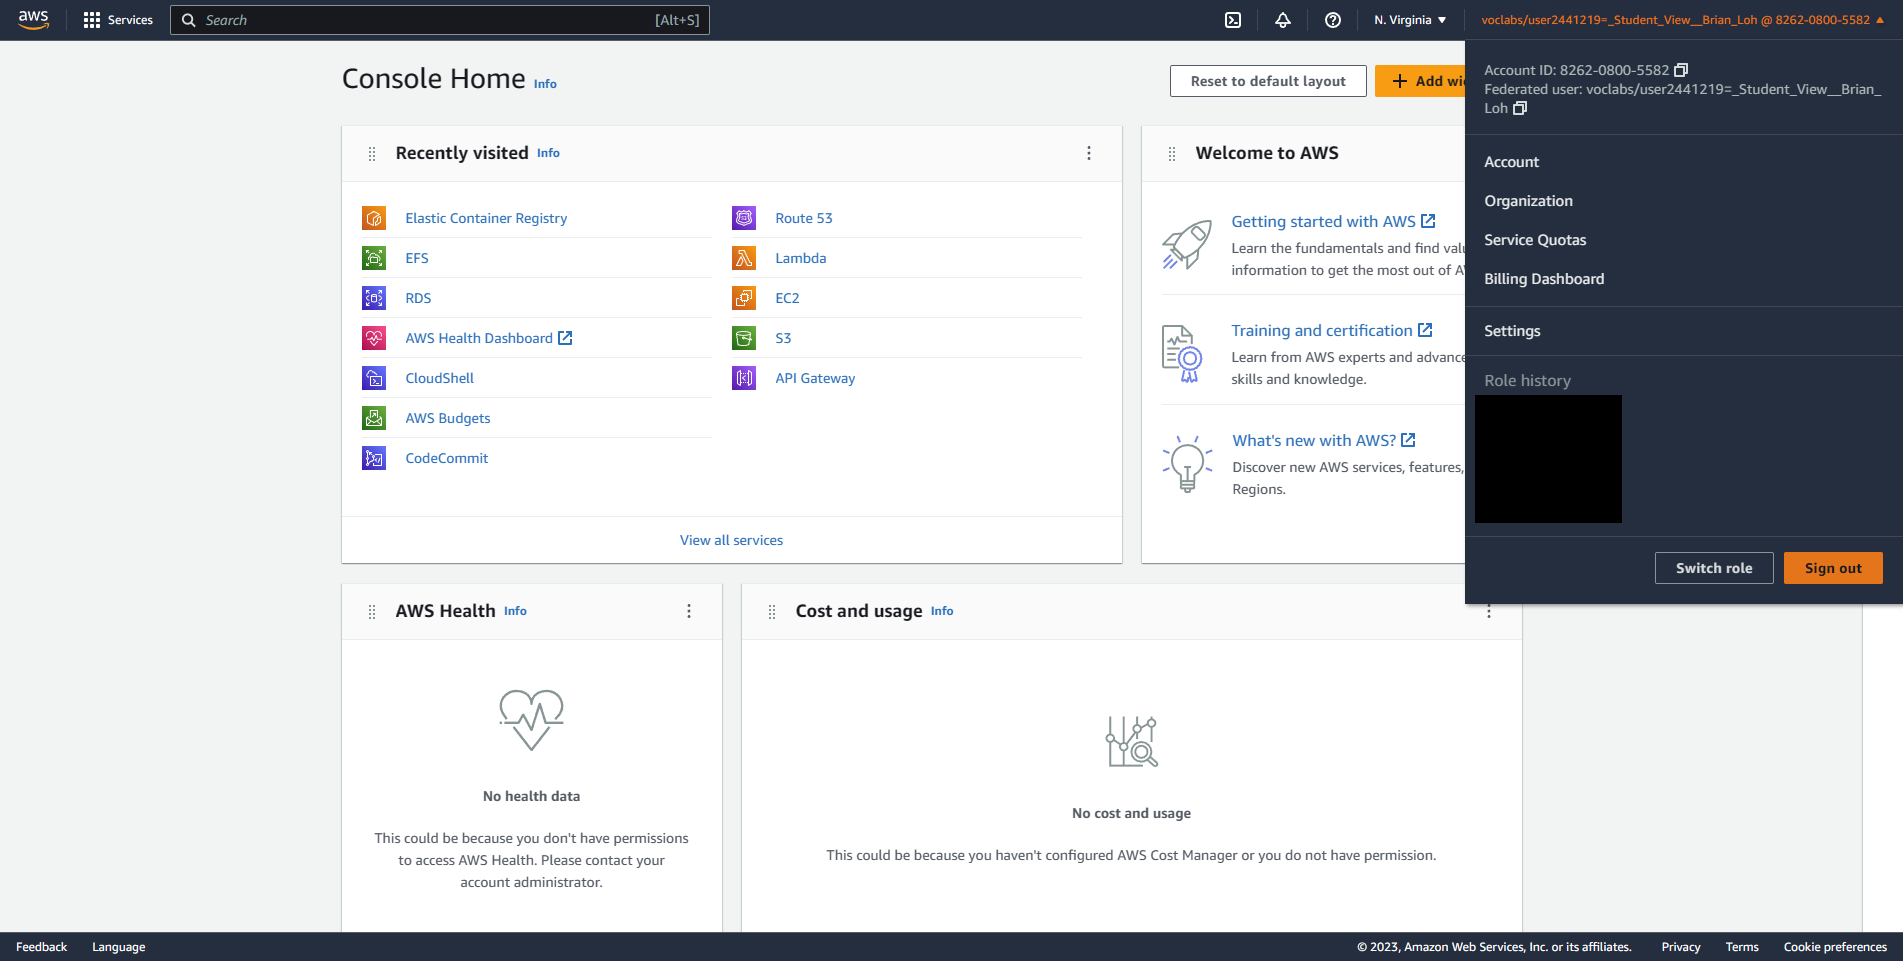
\includegraphics[width=6.2in]{pics/pic.png}
\end{figure}


\vspace{1.5cm}

\newpage

\noindent\underline{VPC setup}

\begin{enumerate}
    \item Paste screenshot$($s$)$ of the \textbf{Your VPCs} screen (before new VPC is created) \\
    \vspace{5mm}
    
    
    {\centering
    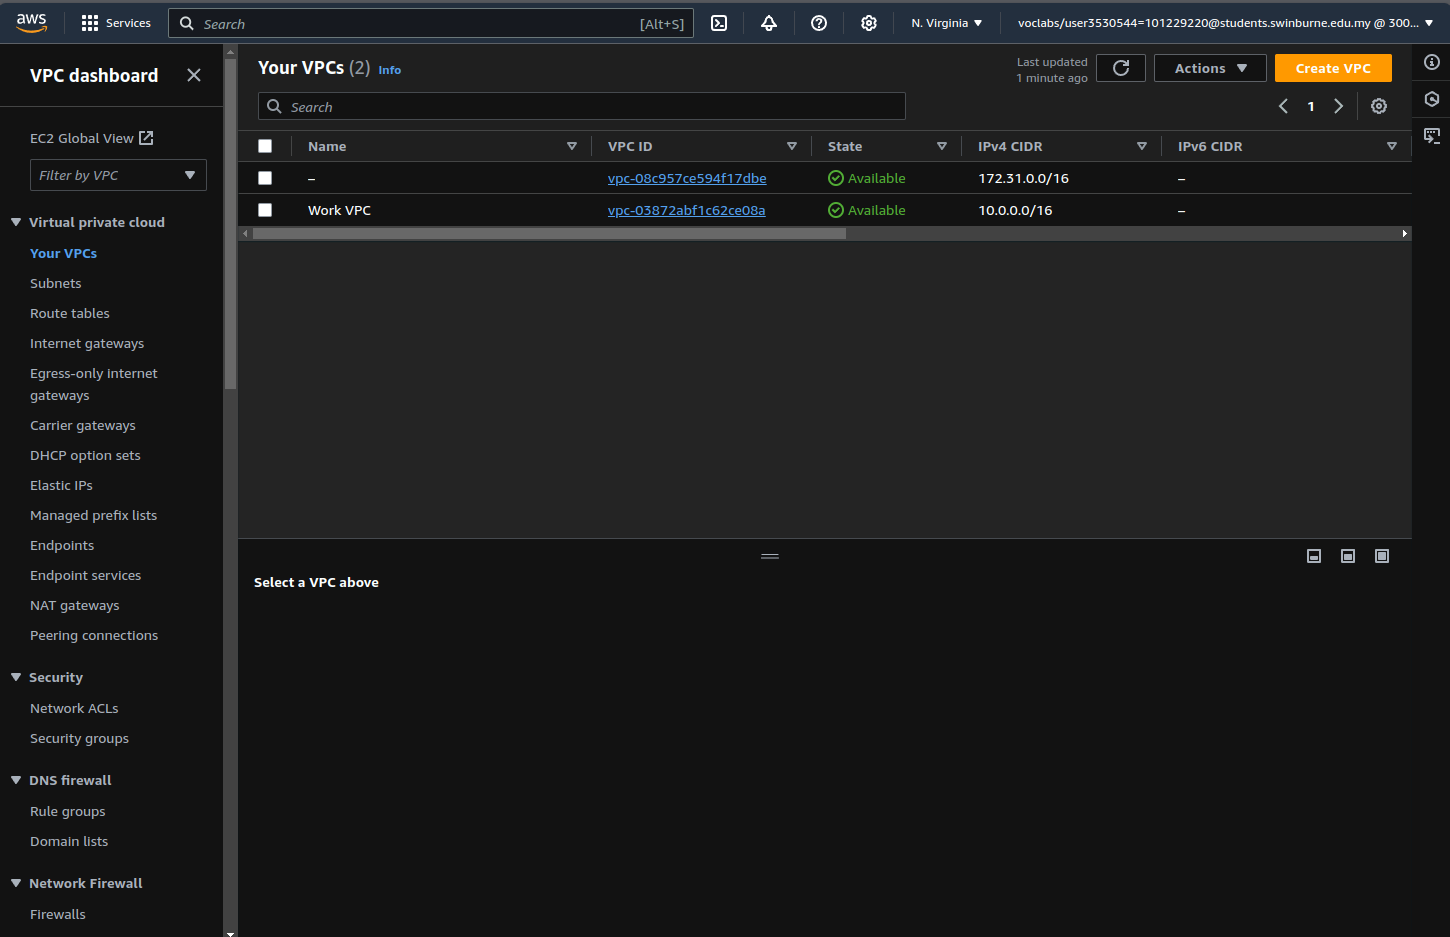
\includegraphics[width=5.8in]{pics/1.png}
    }
    
    \item Paste screenshot$($s$)$ of the \textbf{Create VPC} screen (after entering / choosing the appropriate settings) \\
    \vspace{5mm}

    {\centering
    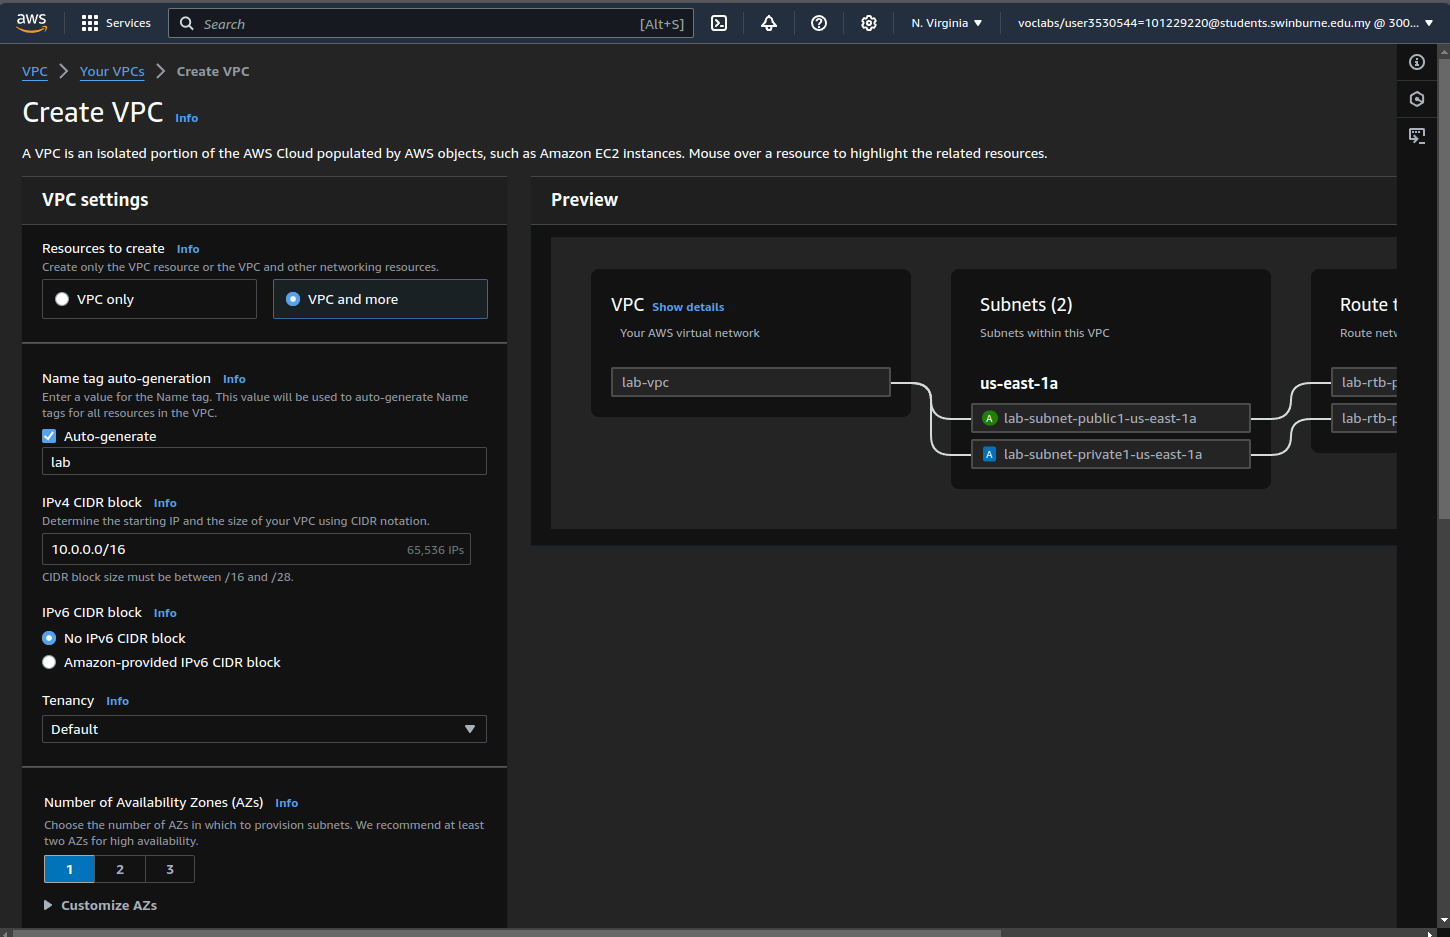
\includegraphics[width=5.8in]{pics/2_a.png}
    }

    \item Paste screenshot$($s$)$ of the \textbf{Your VPCs} screen (after new VPC is created) \\
    \vspace{5mm}

    {\centering
    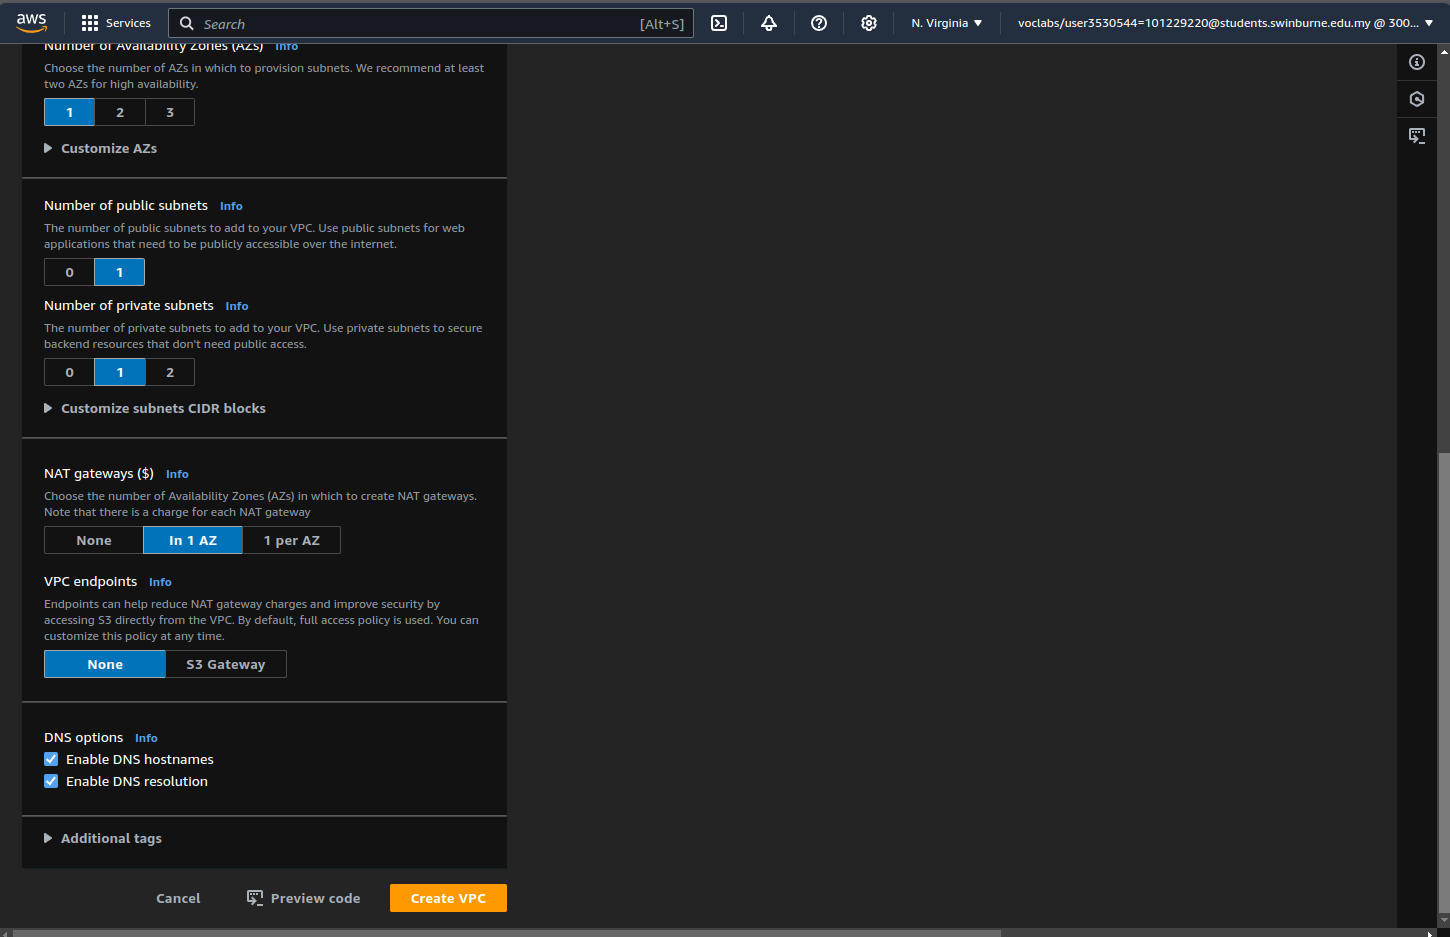
\includegraphics[width=5.8in]{pics/2_b.png}
    }

    \item Paste screenshot$($s$)$ of the \textbf{Subnets} screen (show Public Subnet 1 details) \\
    \vspace{5mm}


    \item Paste screenshot$($s$)$ of the \textbf{Subnets} screen (show Public Subnet 2 details) \\
    \vspace{5mm}


    \item Paste screenshot$($s$)$ of the \textbf{Subnets} screen (show Public Subnet 1 details) \\
    

    \item Paste screenshot$($s$)$ of the \textbf{Subnets} screen (show Public Subnet 2 details) \\
    {\centering
    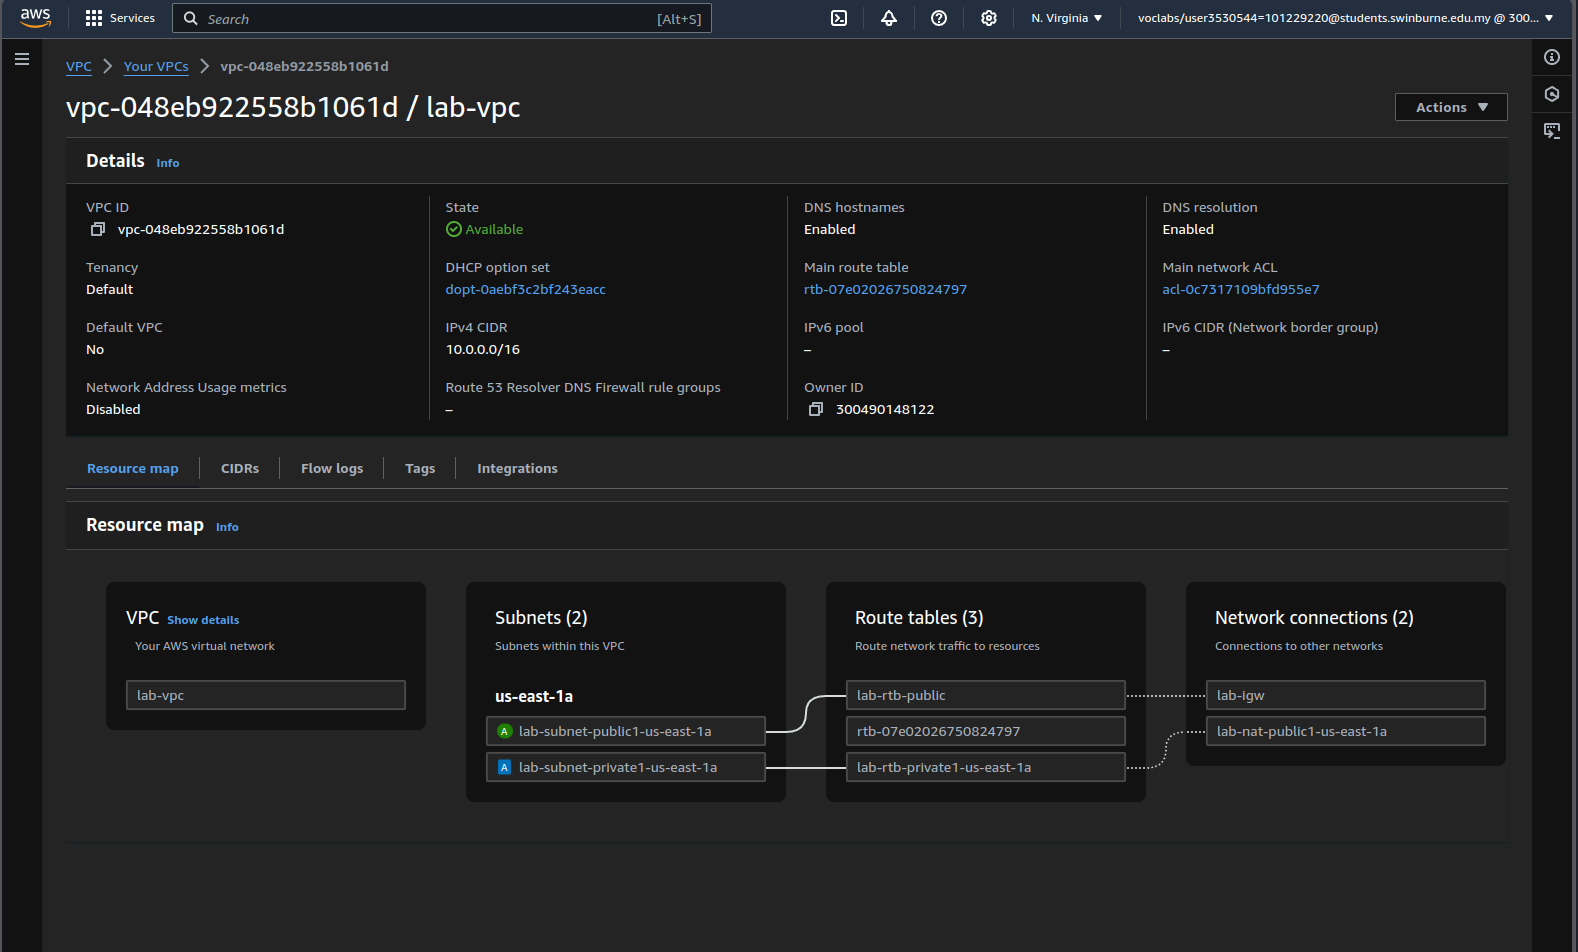
\includegraphics[width=5.8in]{pics/3.png}
    }

    \item Paste screenshot$($s$)$ of the \textbf{Route tables} screen (showing Public Route table routes and subnet associations) \\

    {\centering
    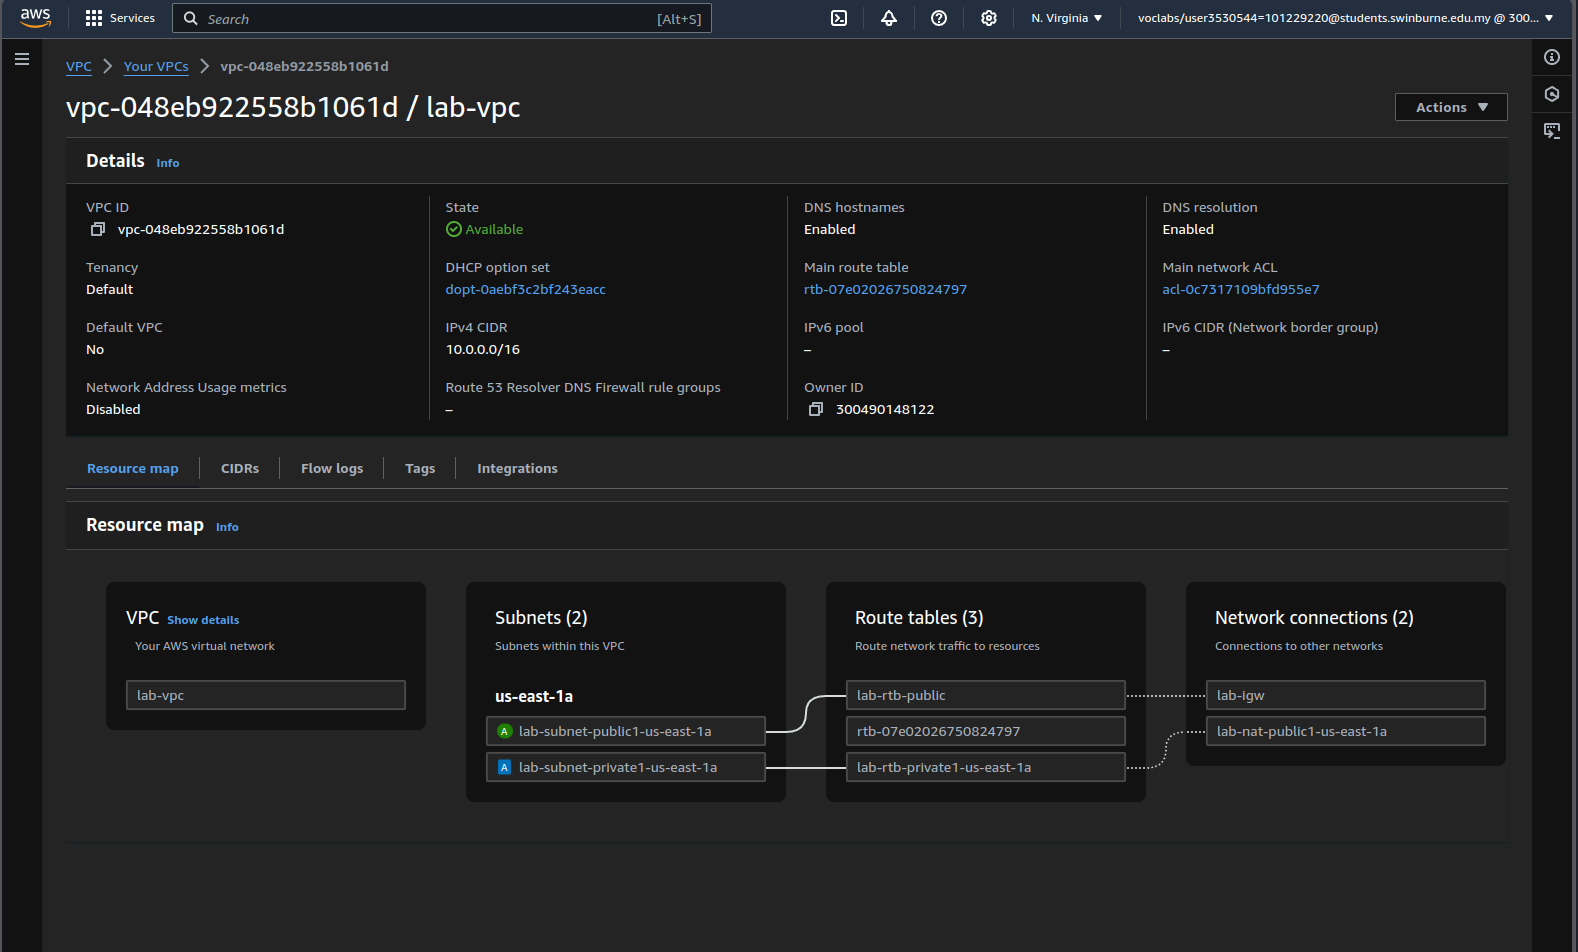
\includegraphics[width=5.8in]{pics/3.png}
    }

    \item Paste screenshot$($s$)$ of the \textbf{Route tables} screen (showing Private Route table routes and subnet associations) \\

    {\centering
    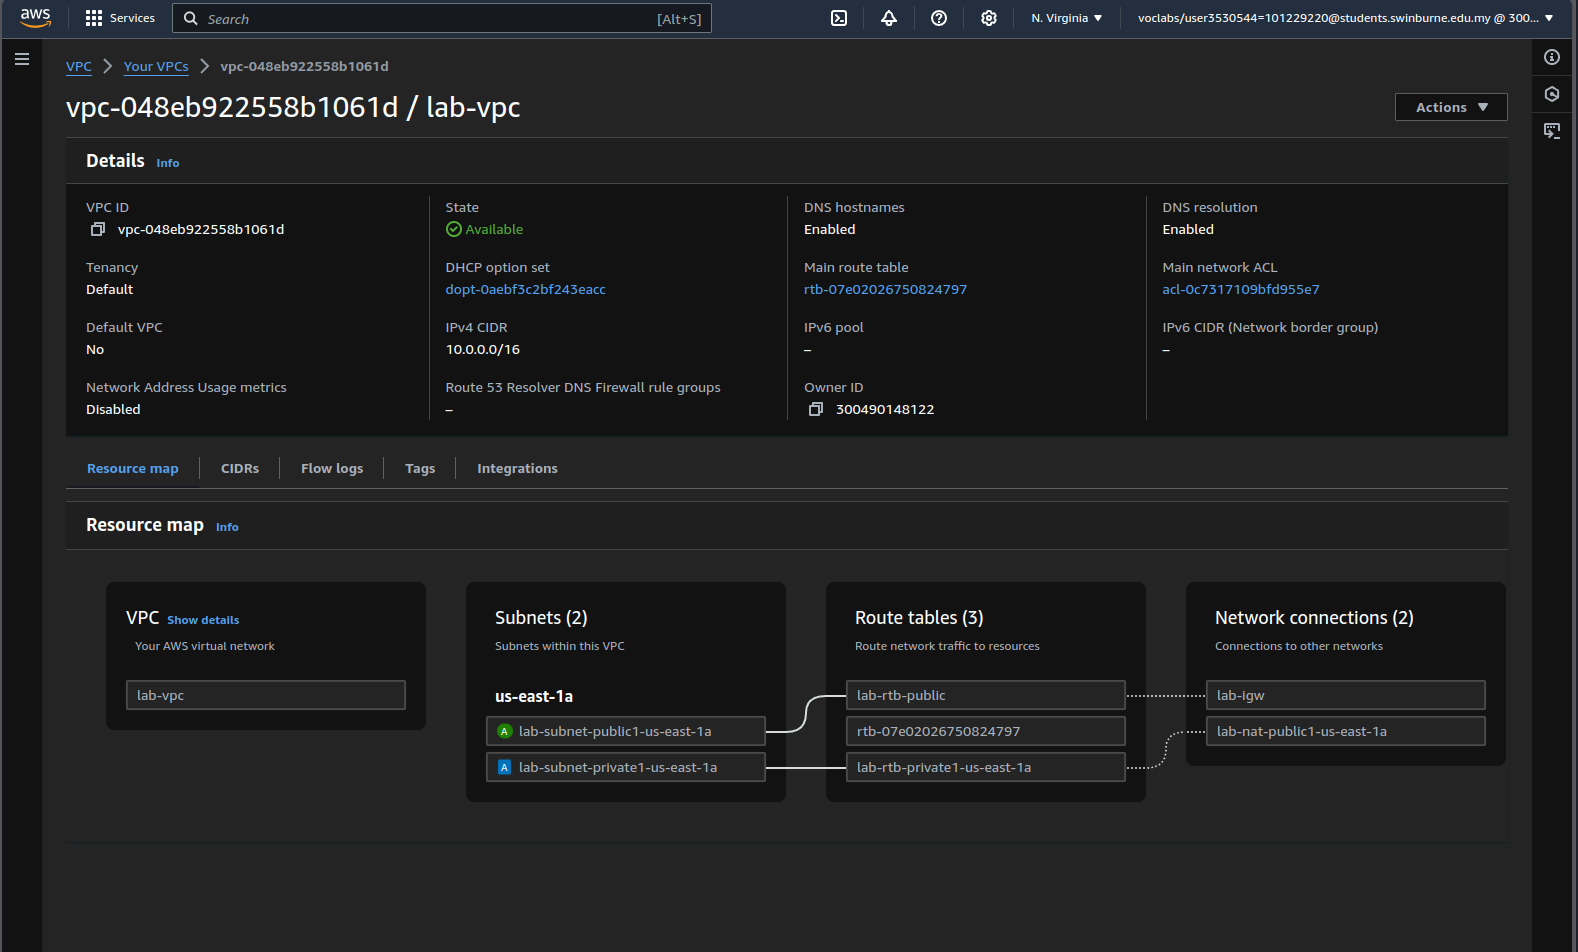
\includegraphics[width=5.8in]{pics/3.png}
    }

\end{enumerate}


\vspace{1cm}

\newpage

\noindent\underline{Security group setup}
\begin{enumerate}[resume]
    \item Paste screenshot$($s$)$ of the \textbf{Security Groups} screen \\

    \item Paste screenshot$($s$)$ of the \textbf{Security Groups} screen (after you have set the Test Tier\\ Security Group configuration)\\
    \vspace{5mm}

    {\centering
    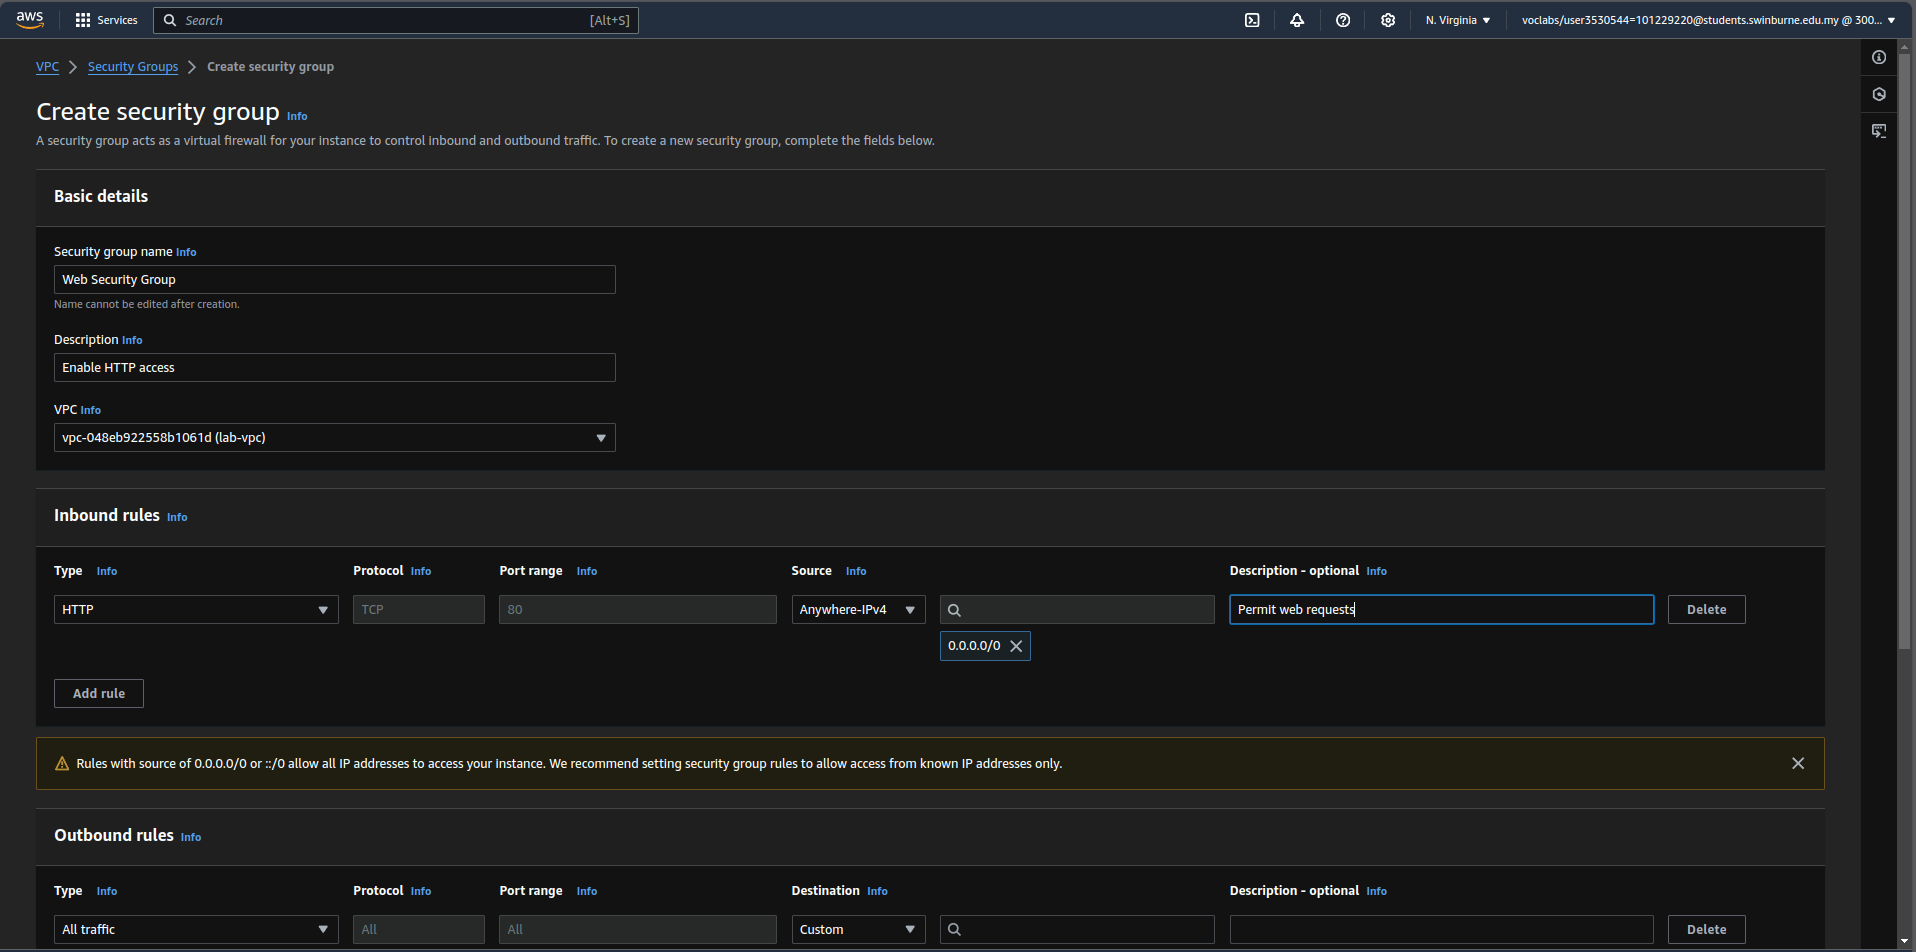
\includegraphics[width=5.8in]{pics/11.png}
    }


    \item Paste screenshot$($s$)$ of the \textbf{Security Groups} screen (after you have set the Web Tier \\ Security Group configuration)\\


    \item Paste screenshot$($s$)$ of the \textbf{Security Groups} screen (after you have set the Database Tier\\ Security Group configuration) \\
    
    \item Paste screenshot$($s$)$ of the \textbf{Create Security Group} screen  \\
    \vspace{5mm}

    {\centering
    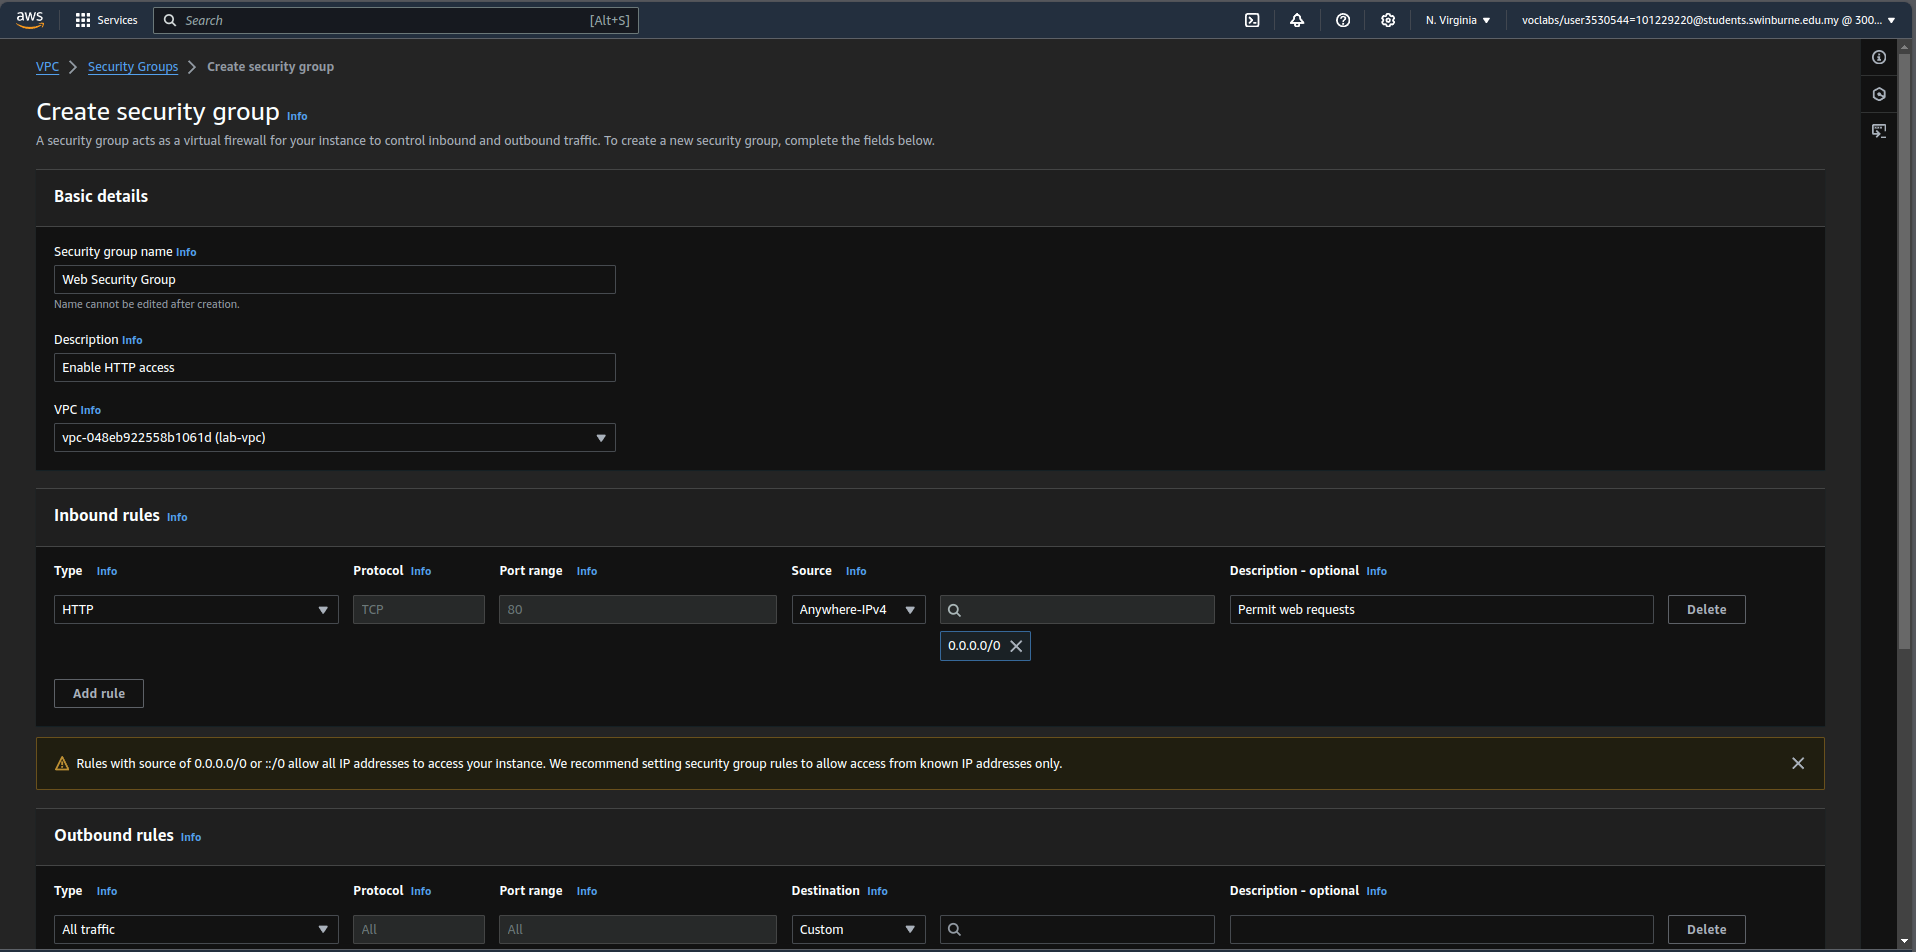
\includegraphics[width=5.8in]{pics/12_a.png}
    }

\end{enumerate}


\newpage

\noindent\underline{EC2 setup (Web Server)}
\begin{enumerate}[resume]
    \item Paste screenshot$($s$)$ of the \textbf{Launch an instance – Name and tags} screen (after entering / choosing the appropriate settings) \\
    \vspace{5mm}

    {\centering
    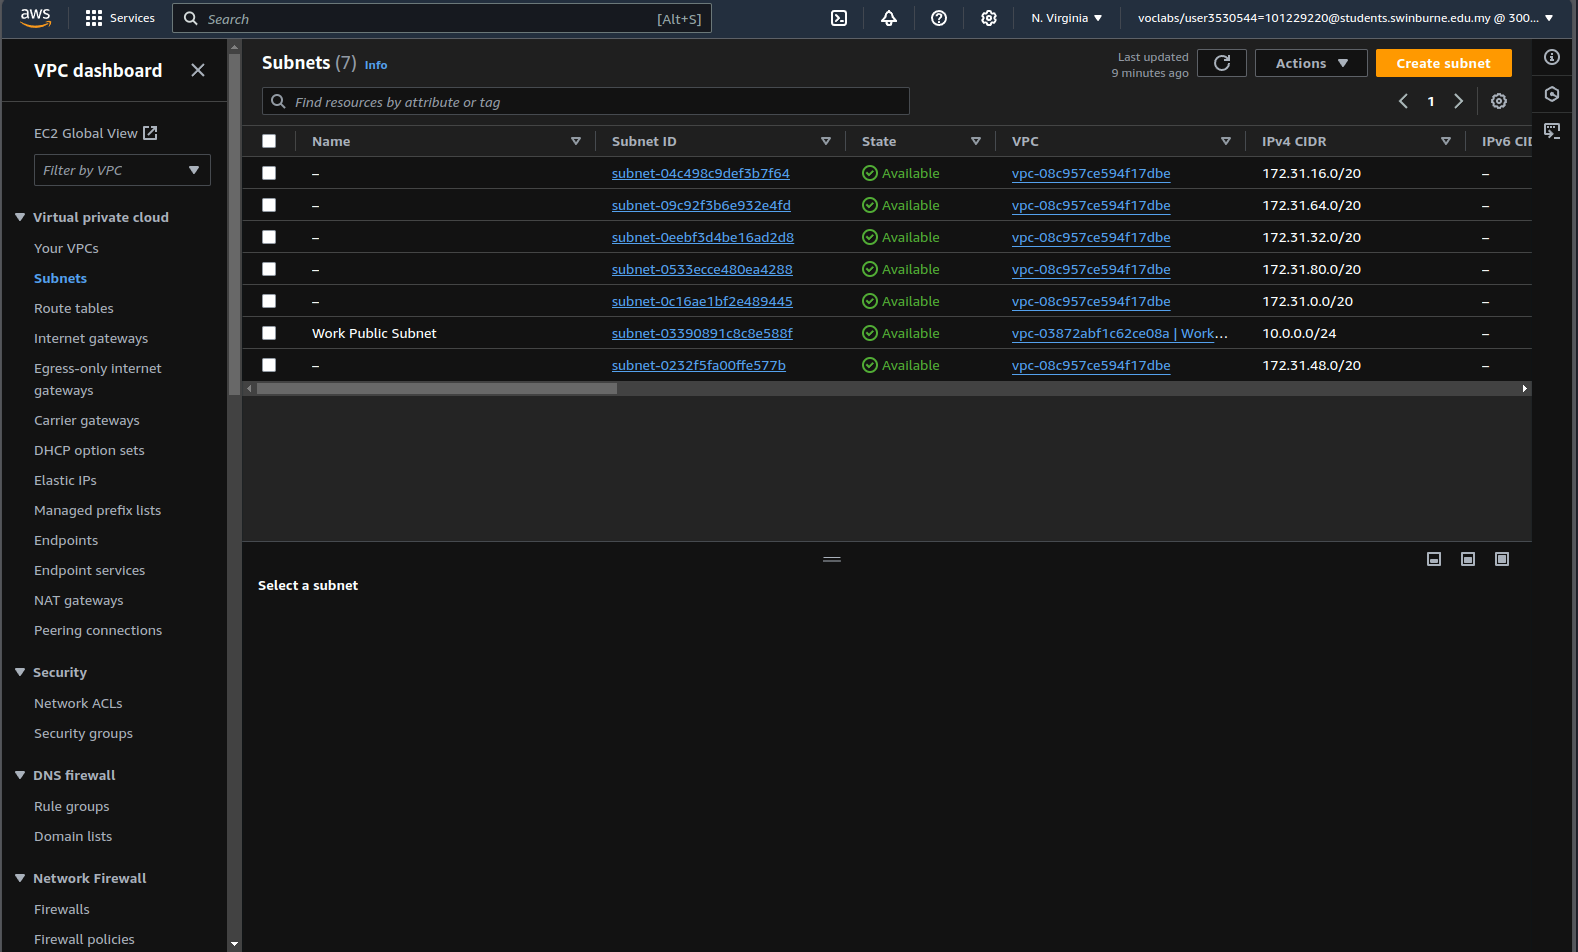
\includegraphics[width=5.8in]{pics/4.png}
    }


    \item Paste screenshot$($s$)$ of the \textbf{Launch an instance – Application and OS images} screen (after entering / choosing the appropriate settings) \\
    \vspace{5mm}

    {\centering
    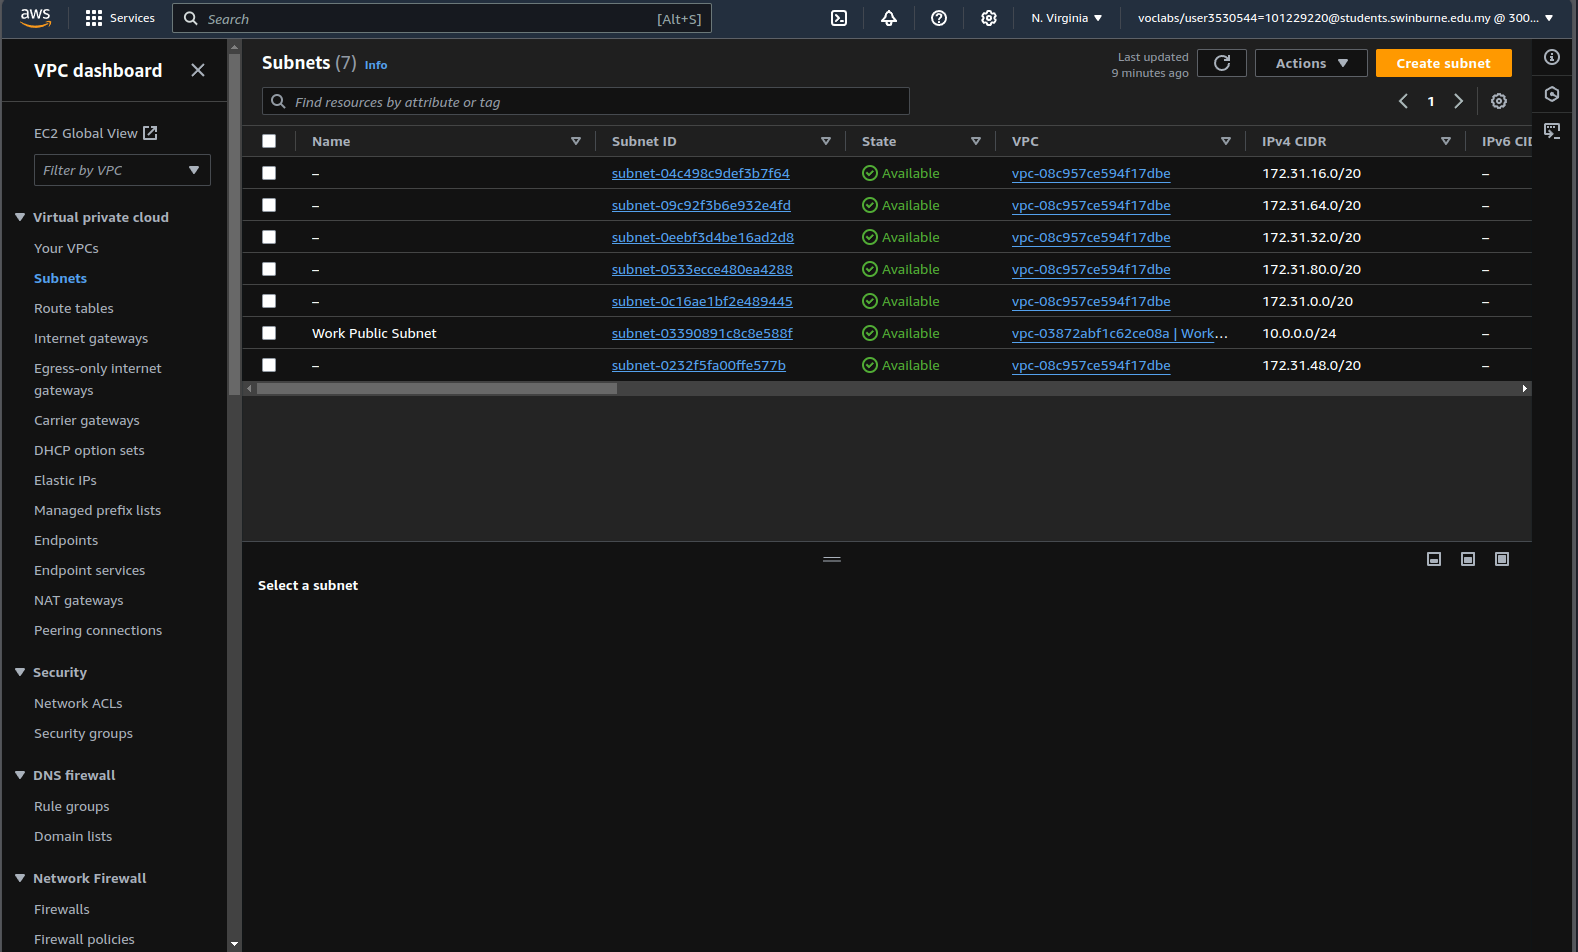
\includegraphics[width=5.8in]{pics/4.png}
    }


    \item Paste screenshot$($s$)$ of the \textbf{Launch an instance – Instance type} screen (after entering / choosing the appropriate settings) \\
    \vspace{5mm}

    {\centering
    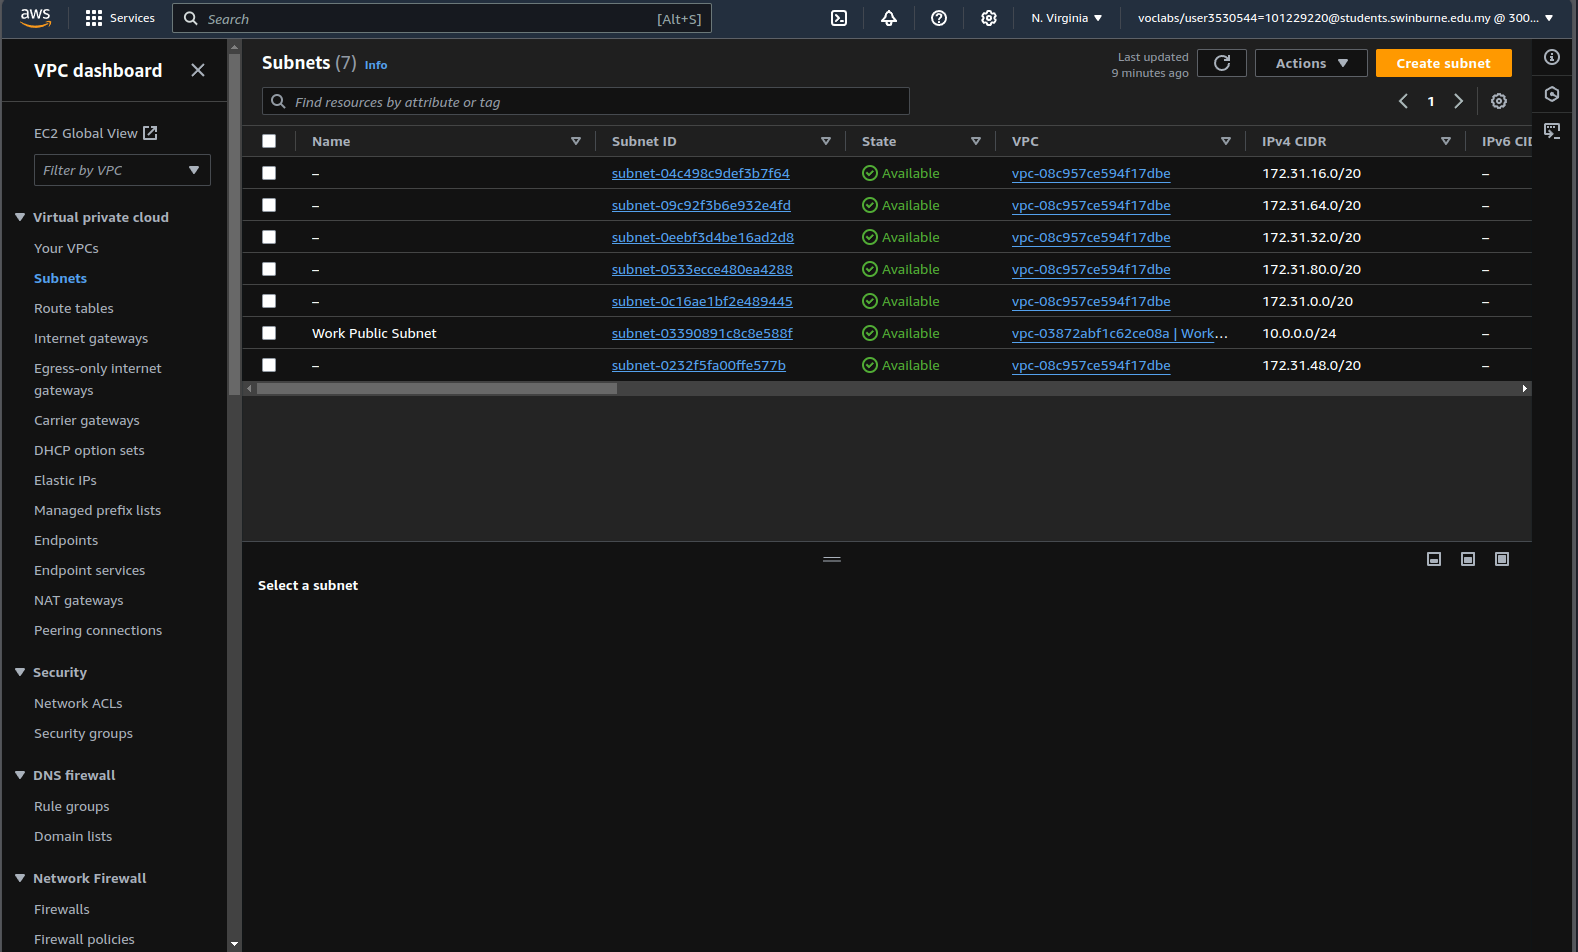
\includegraphics[width=5.8in]{pics/4.png}
    }



    \item Paste screenshot$($s$)$ of the \textbf{Launch an instance – Key pair} screen (after entering / choosing the appropriate settings) \\
    \vspace{5mm}

    {\centering
    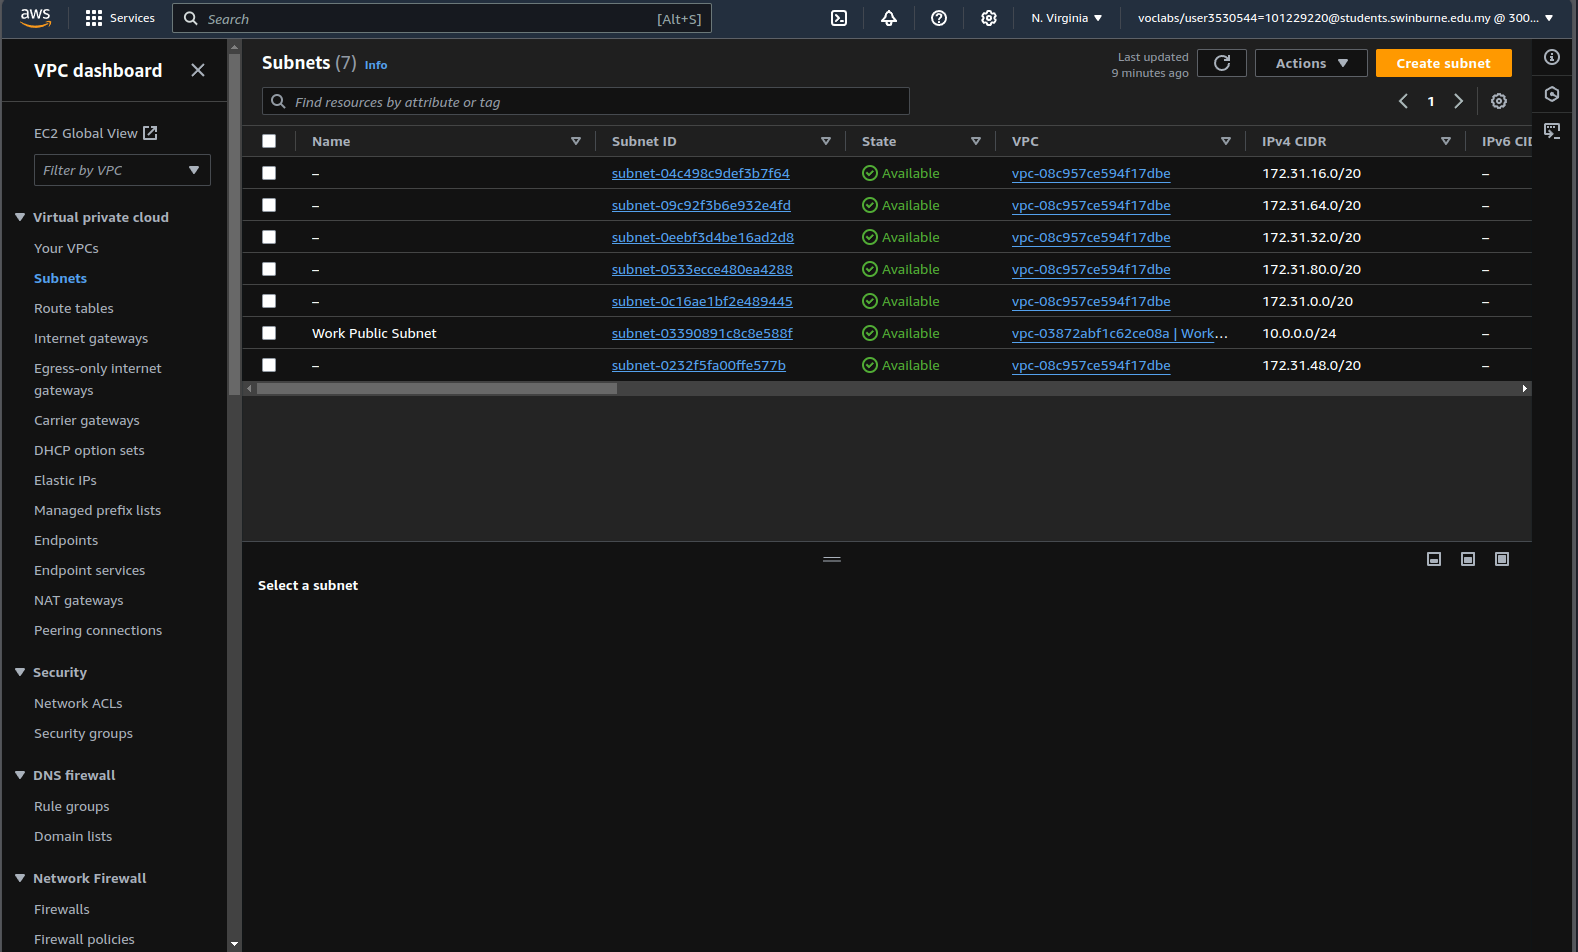
\includegraphics[width=5.8in]{pics/4.png}
    }



    \item Paste screenshot$($s$)$ of the \textbf{Launch an instance – Network settings} screen (after entering / choosing the appropriate settings) \\
    \vspace{5mm}

    {\centering
    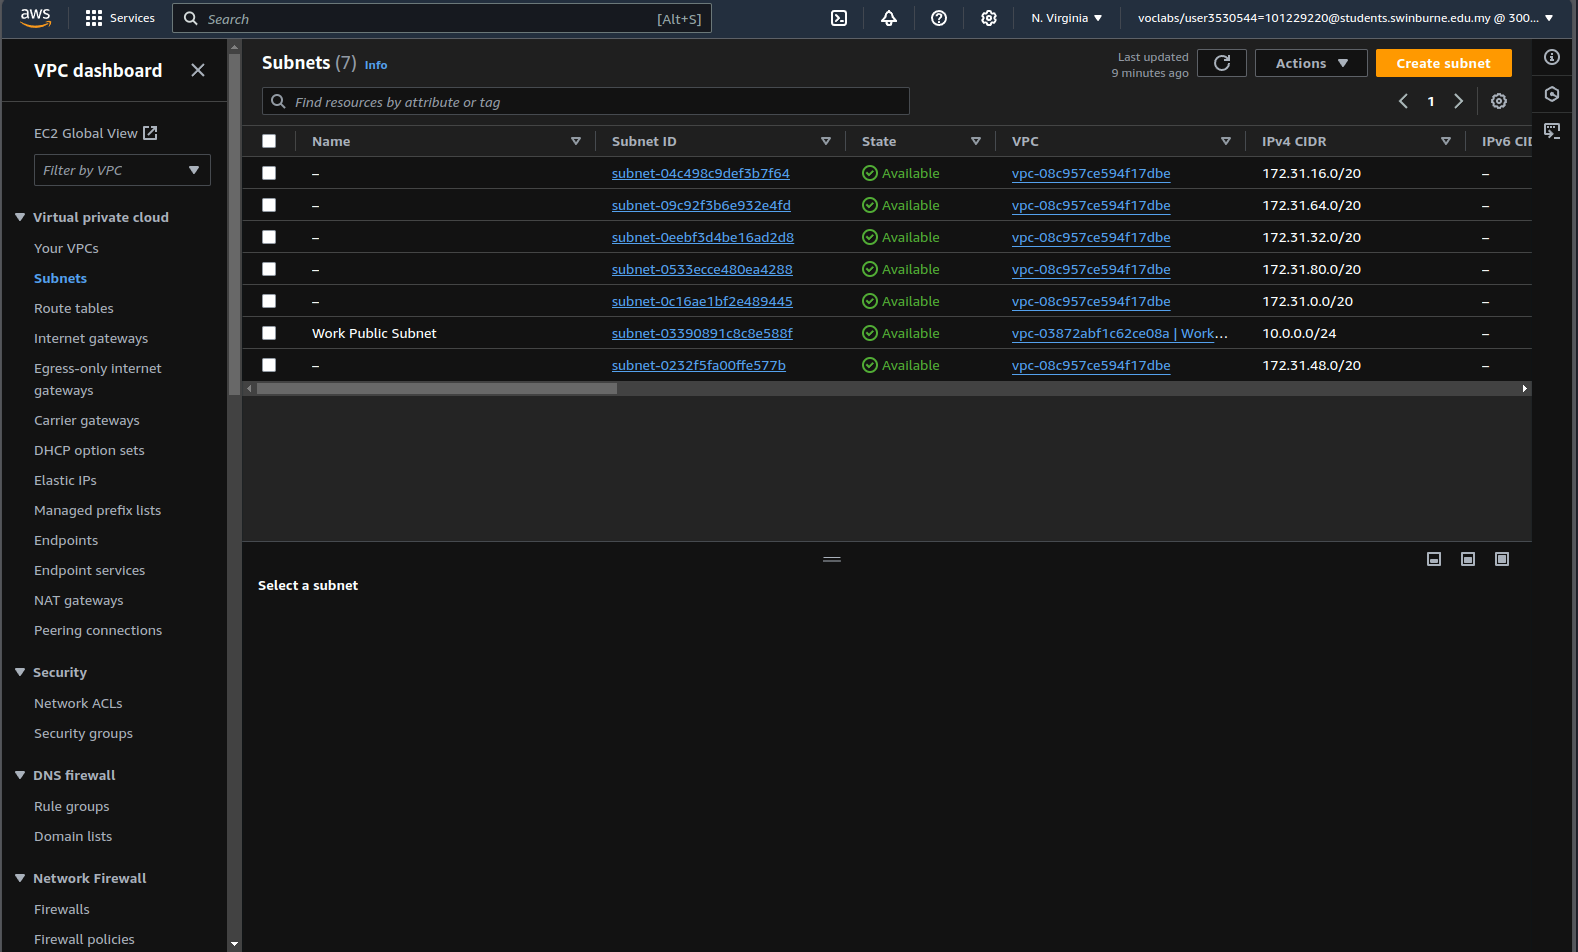
\includegraphics[width=5.8in]{pics/4.png}
    }


    \item Paste screenshot$($s$)$ of the \textbf{Launch an instance – Configure storage} screen (after entering / choosing the appropriate settings) \\
    \vspace{5mm}

    {\centering
    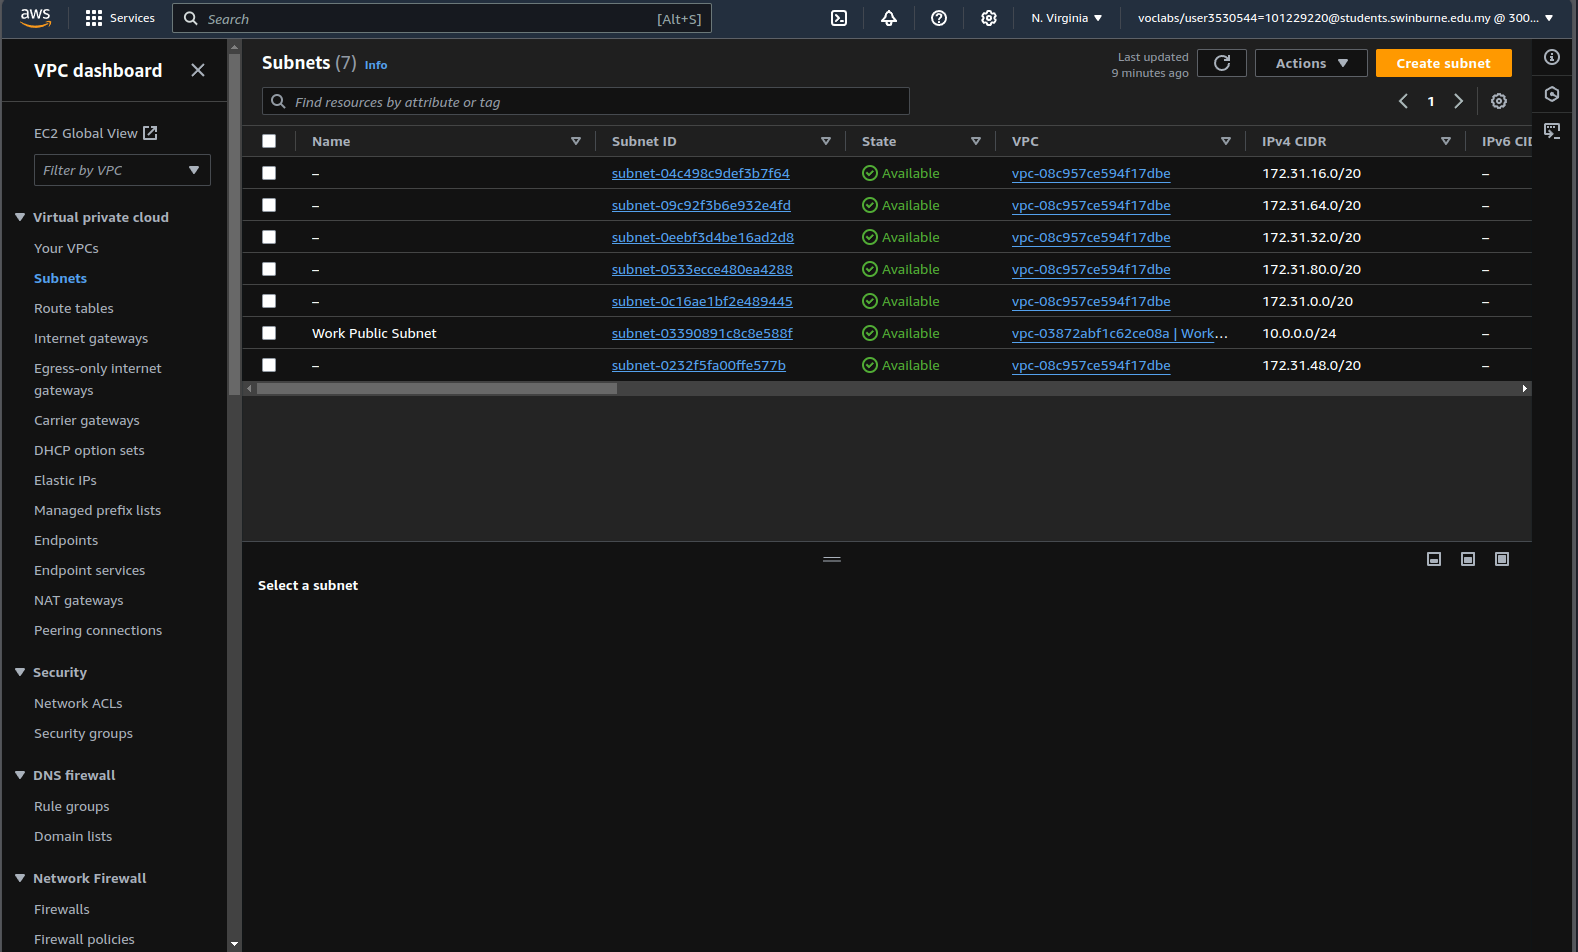
\includegraphics[width=5.8in]{pics/4.png}
    }



    \item Paste screenshot$($s$)$ of the \textbf{Launch an instance – Advanced details} screen (after entering / choosing the appropriate settings) \\
    \vspace{5mm}

    {\centering
    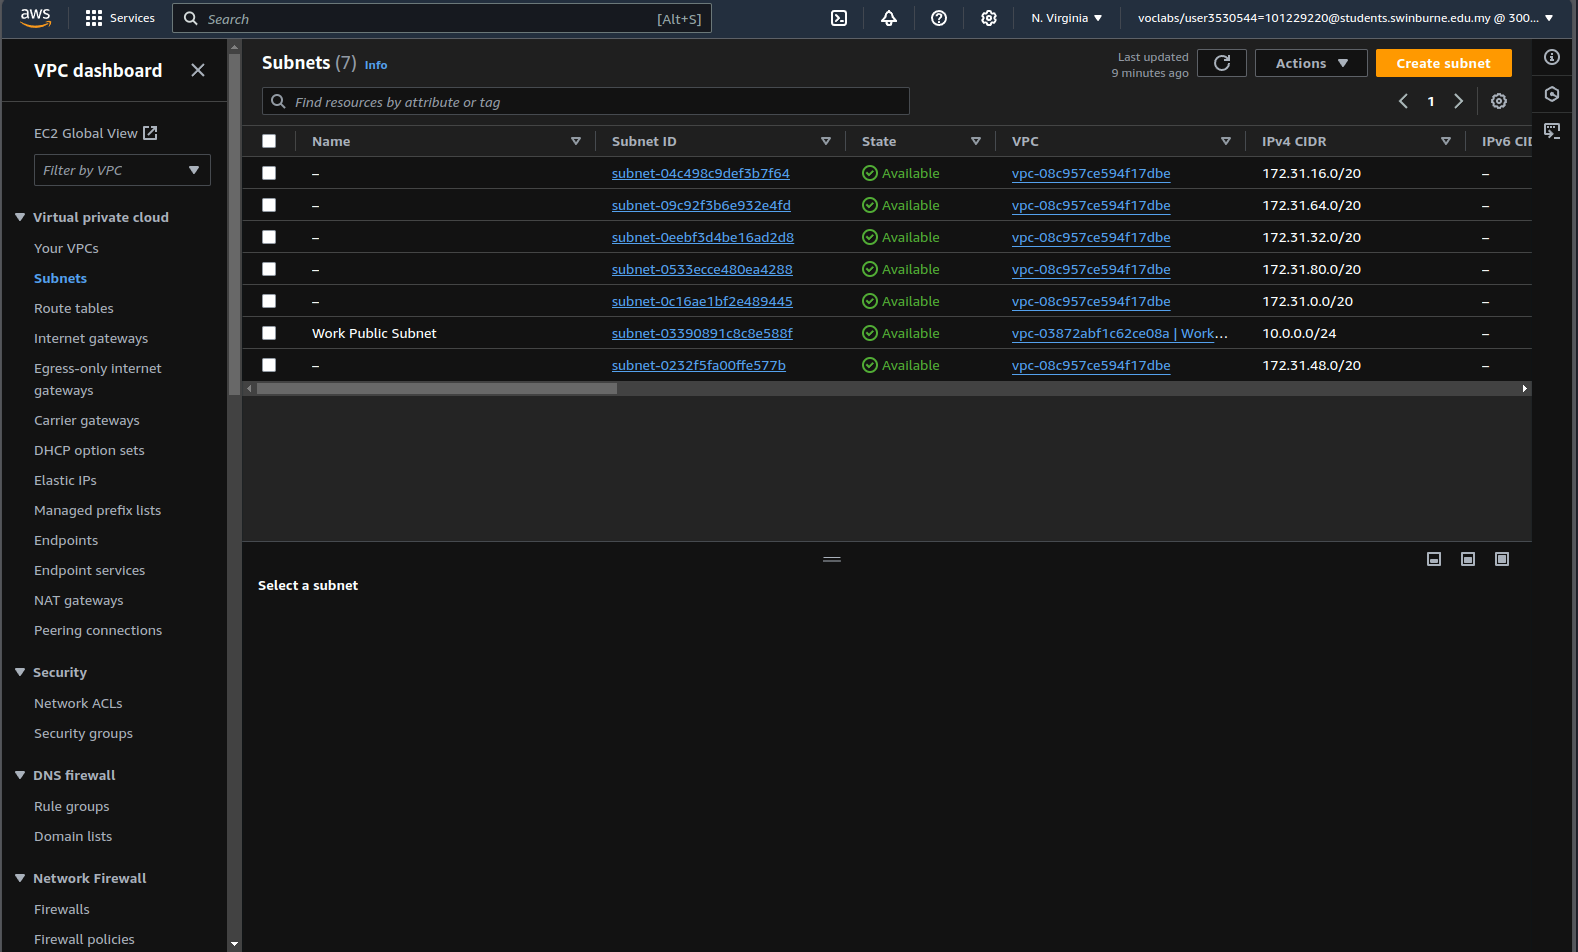
\includegraphics[width=5.8in]{pics/4.png}
    }



    \item Paste screenshot$($s$)$ of the \textbf{Instances} screen (show your running server and the IP address) \\
    \vspace{5mm}

    {\centering
    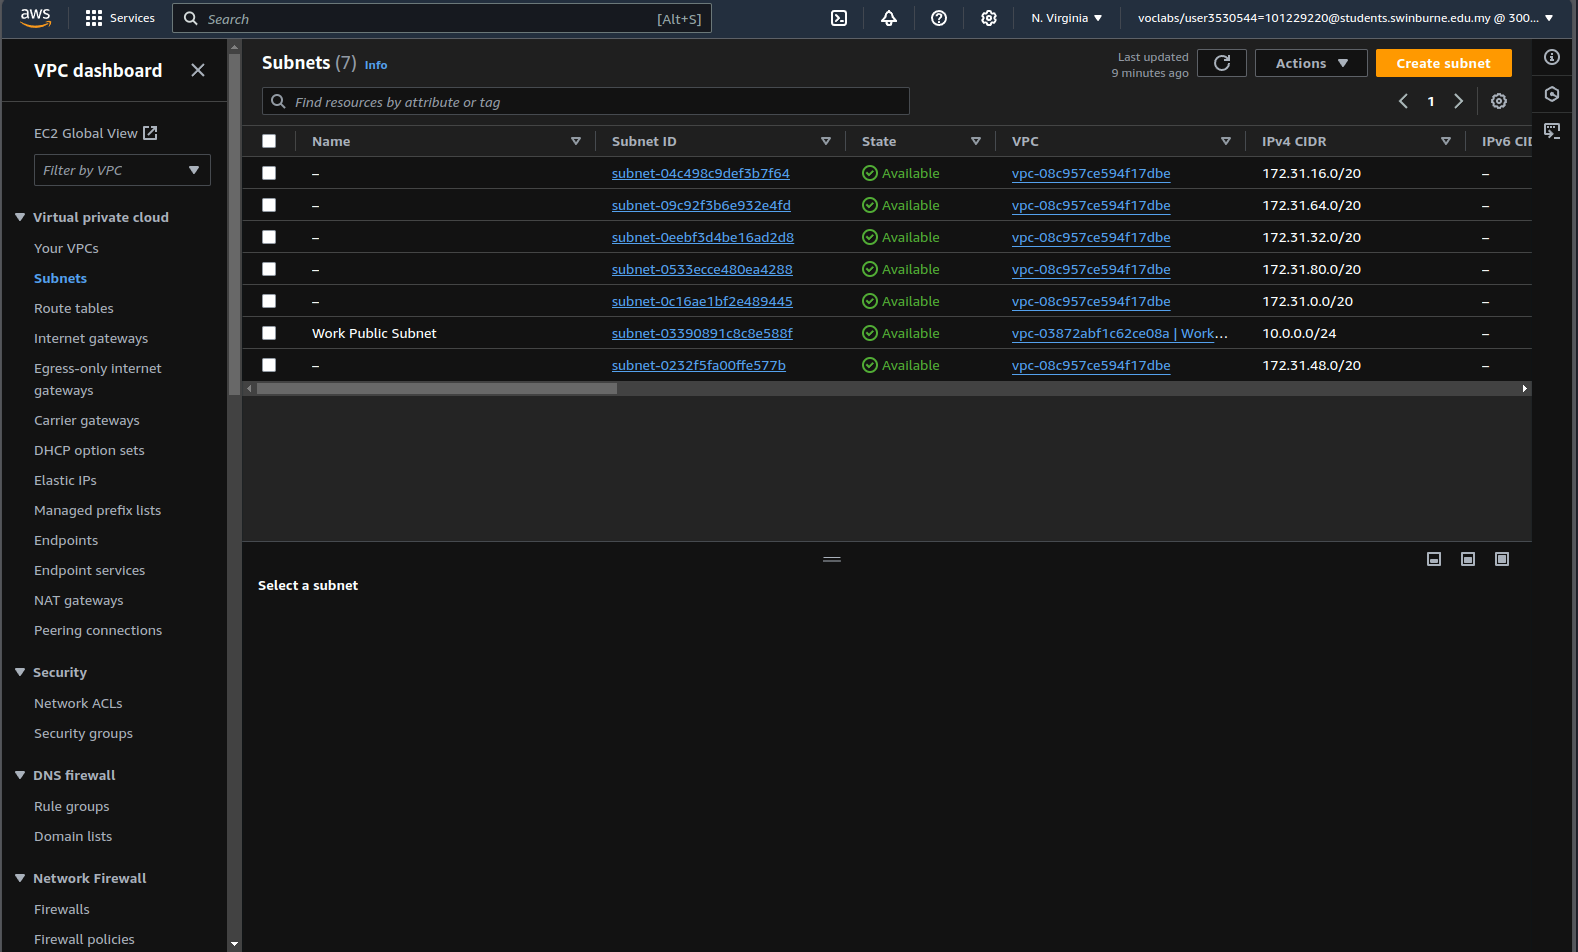
\includegraphics[width=5.8in]{pics/4.png}
    }
\end{enumerate}




\newpage
\noindent\underline{RDS setup}    
\begin{enumerate}[resume]
    \item Paste screenshot$($s$)$ of the \textbf{Subnet groups} screen (before subnet group is created) \\
    
    \vspace{2mm}
    
    \item Paste screenshot$($s$)$ of the \textbf{Create DB subnet group} screen (after entering / choosing the \\ appropriate settings) \\
    \vspace{2mm}

    {\centering
    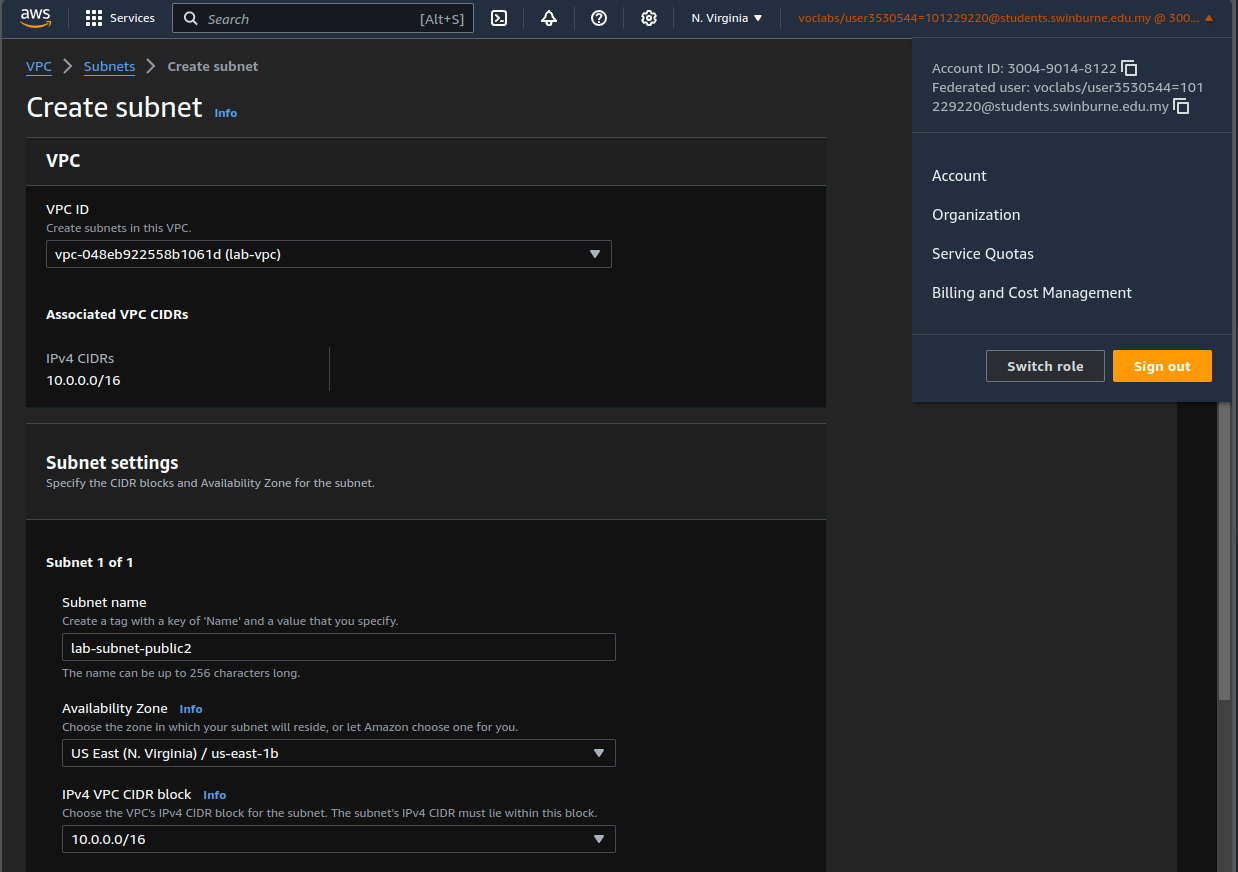
\includegraphics[width=5.8in]{pics/5_a.png}
    }

    
    \item Paste screenshot$($s$)$ of the \textbf{Subnet groups} screen \\
    \vspace{2mm}

    {\centering
    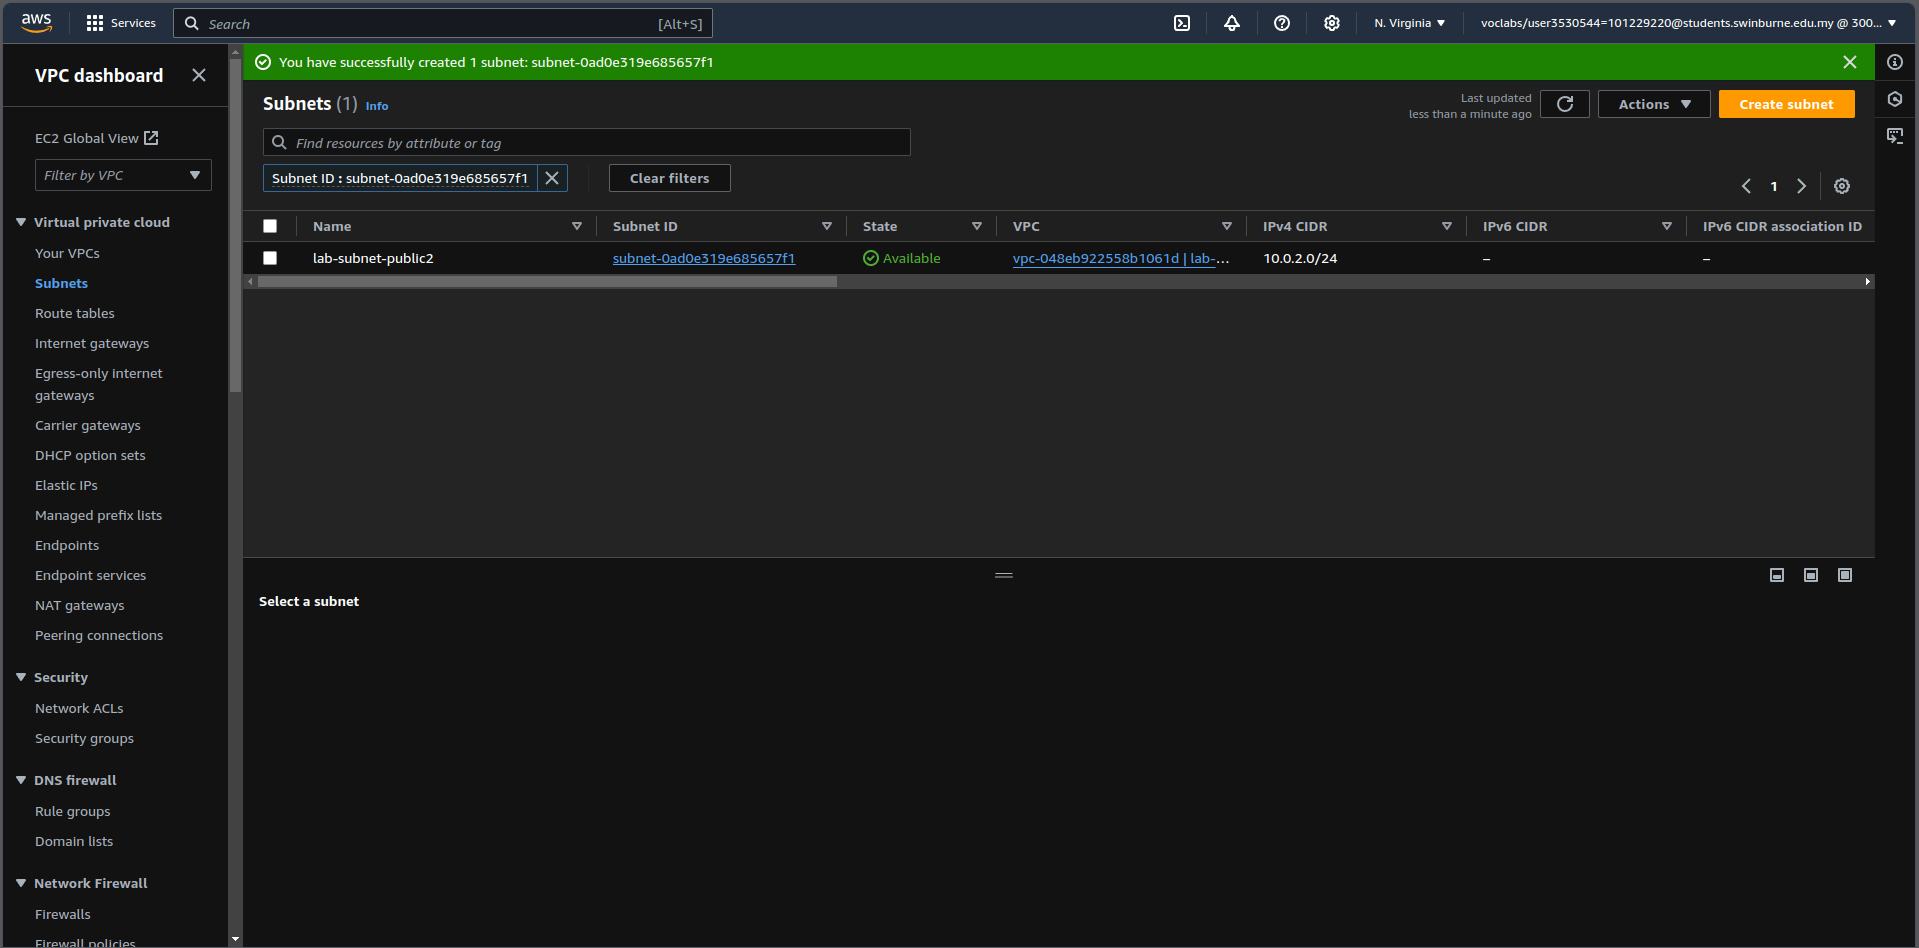
\includegraphics[width=5.8in, height=5.0in]{pics/6.png}
    }
    
    \vspace{50mm}
    \item Paste screenshot$($s$)$ of the \textbf{Create database – Engine options} screen (after entering / choosing the \\ appropriate settings) \\
    \vspace{5mm}

    \item Paste screenshot$($s$)$ of the \textbf{Create database – Settings} screen (after entering / choosing the \\ appropriate settings) \\
    \vspace{5mm}

    \item Paste screenshot$($s$)$ of the \textbf{Create database – Instance configuration} screen (after entering / choosing the \\ appropriate settings) \\
    \vspace{5mm}

    \item Paste screenshot$($s$)$ of the \textbf{Create database – Storage} screen (after entering / choosing the \\ appropriate settings) \\
    \vspace{5mm}
    
    \item Paste screenshot$($s$)$ of the \textbf{Create database – Connectivity} screen (after entering / \\choosing the appropriate settings) \\

    \item Paste screenshot$($s$)$ of the \textbf{Databases} screen \\
    \vspace{0.01mm}
\end{enumerate}




\newpage
\noindent\underline{S3 setup}    
\begin{enumerate}[resume]    
    \item Paste screenshot$($s$)$  of the \textbf{Buckets} screen  \\
    \vspace{5mm}

    {\centering
    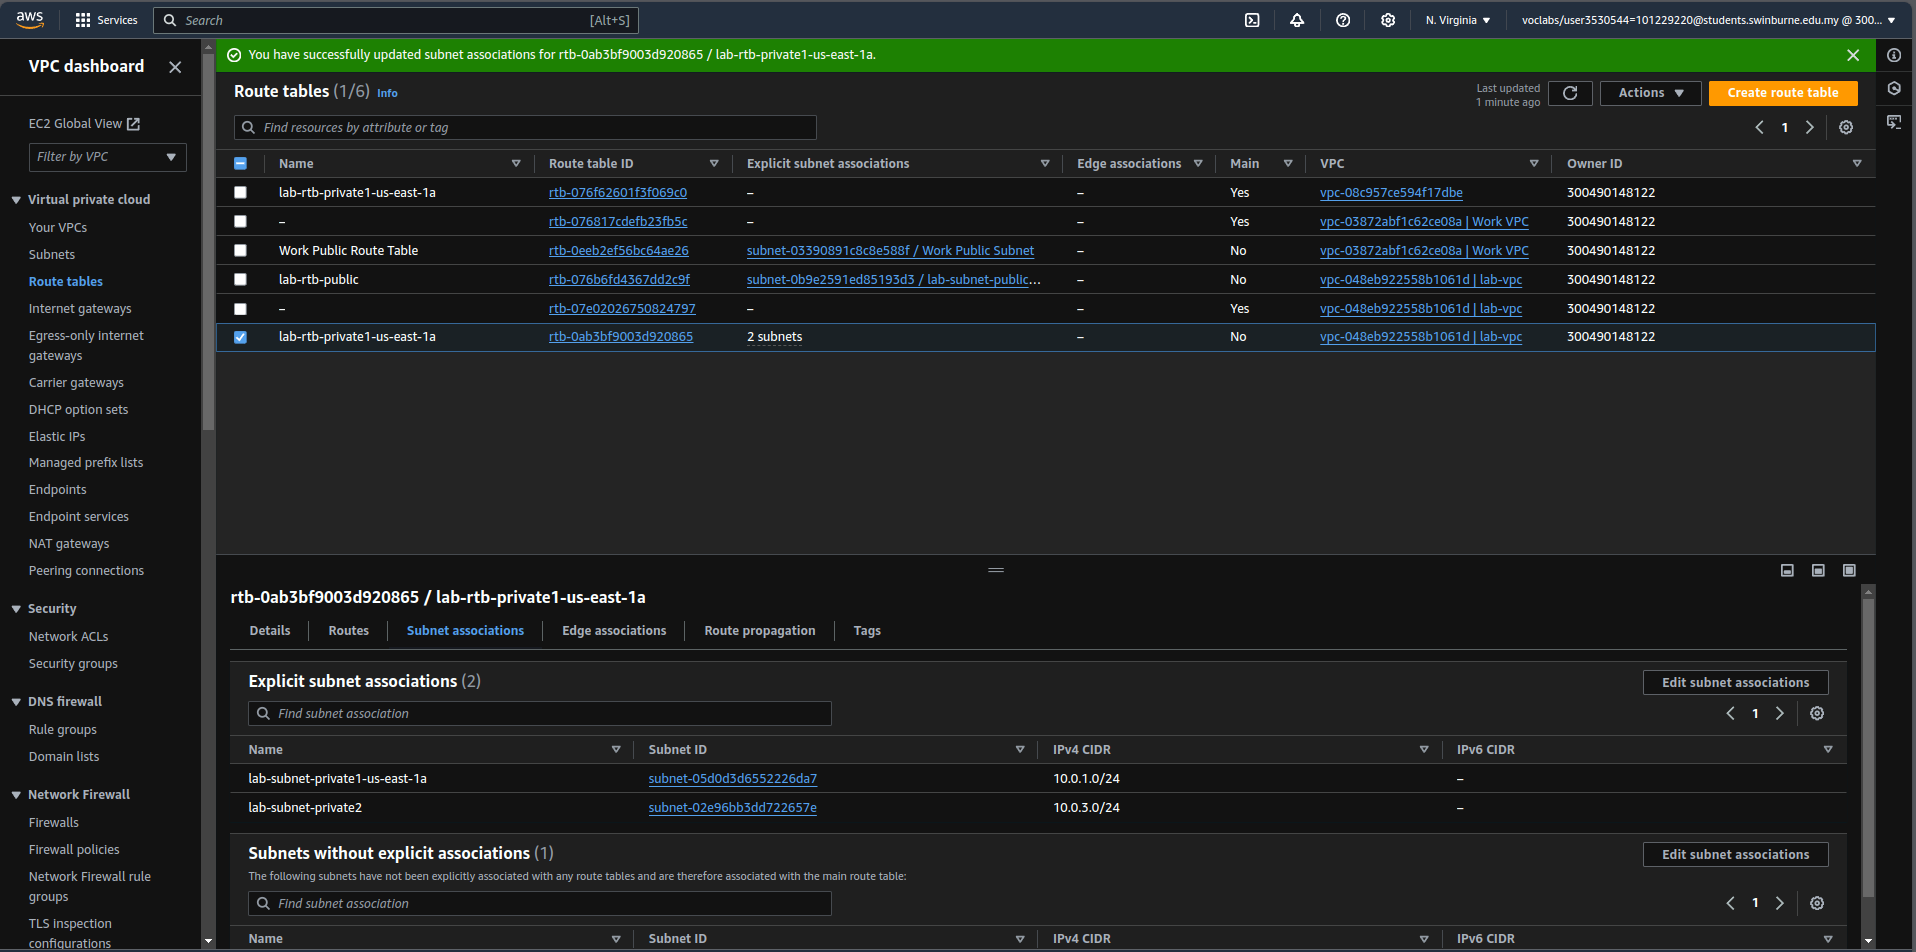
\includegraphics[width=5.8in]{pics/9.png}
    }

    
    \item Paste screenshot$($s$)$ of the \textbf{Create bucket} screen (after entering / choosing the appropriate settings)\\
    \vspace{5mm}

    {\centering
    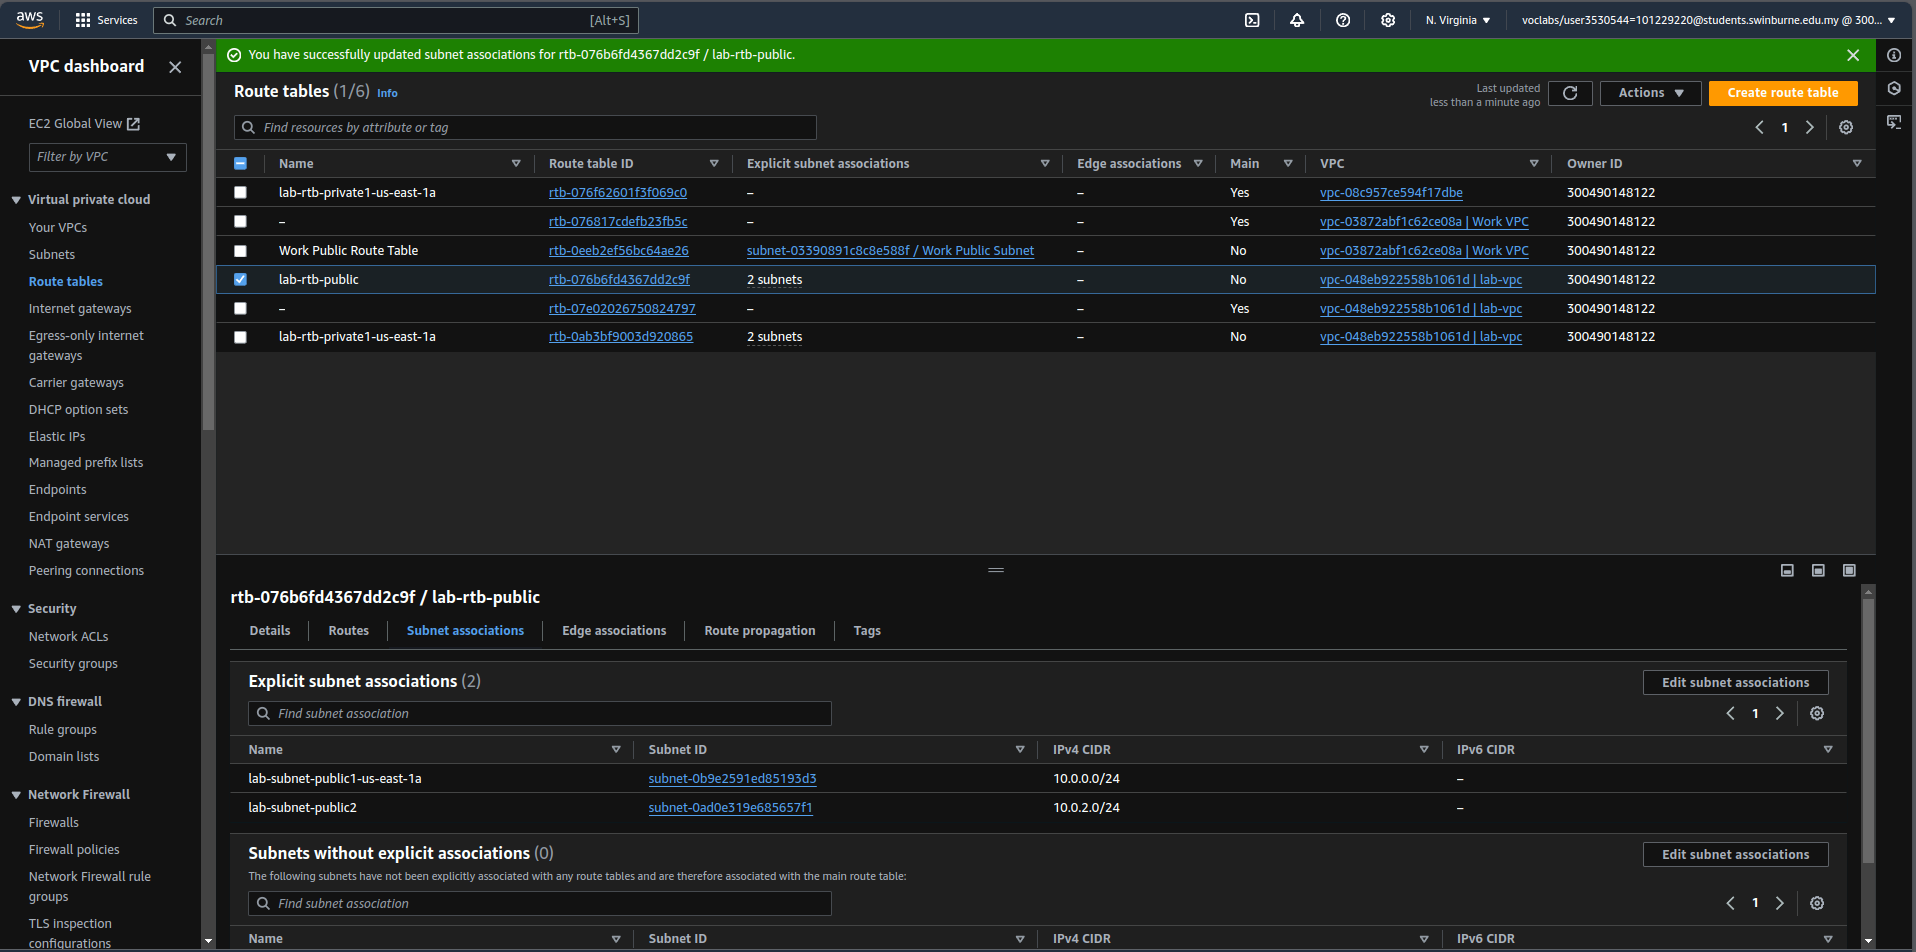
\includegraphics[width=5.8in]{pics/10.png}
    }


    \item Paste screenshot$($s$)$ of the \textbf{Bucket – Permissions} screen (after entering / choosing the appropriate settings)\\

    \item Paste screenshot$($s$)$ of the \textbf{files in the Bucket} \\
\end{enumerate}


\vspace{1cm}

\newpage

\noindent\underline{Database schema}
\begin{enumerate}[resume]
    \item Paste screenshot$($s$)$ of the database schema (e.g.\ entity relationship diagram, SQL code) you have created \\ 
    \vspace{5mm}

    {\centering
    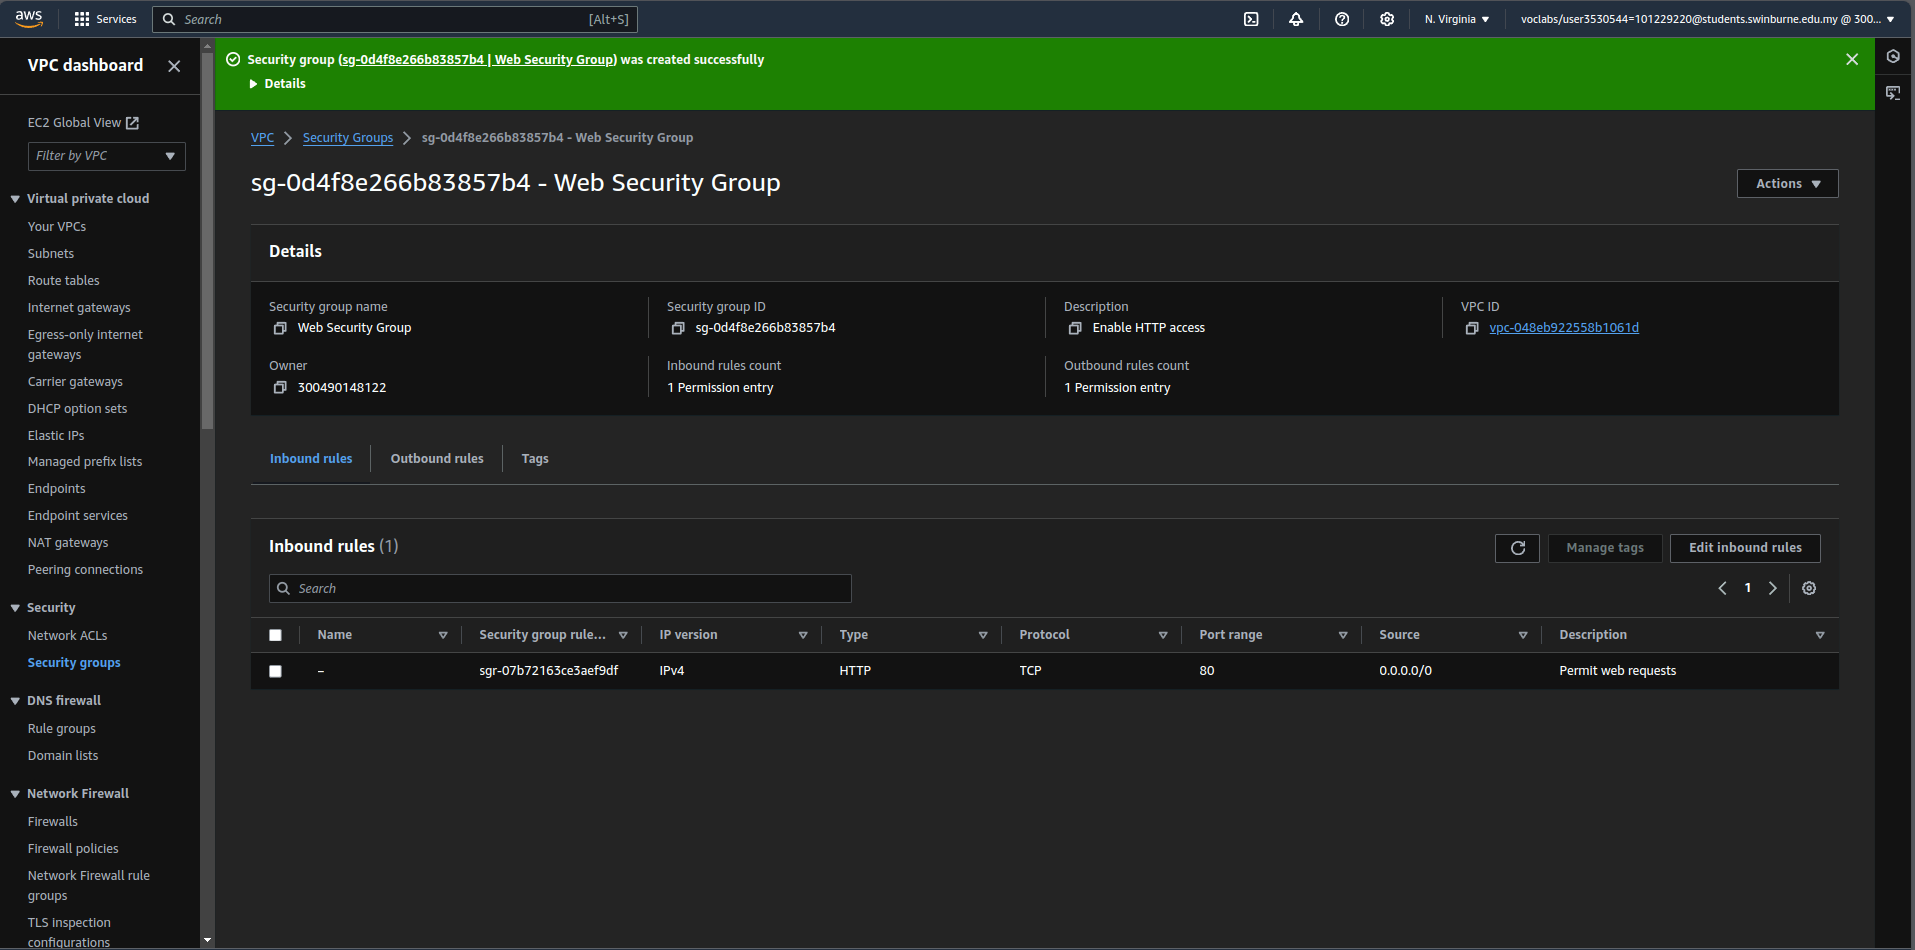
\includegraphics[width=5.8in]{pics/13.png}
    }

    \item Paste screenshot$($s$)$ of how you have accessed and created your database table and records \\
\end{enumerate}

\vspace{0.2cm}

\newpage
\noindent\underline{Website}

\begin{enumerate}[resume]
    \item Paste screenshot$($s$)$ of the \textbf{get\_files.php} source code \\
    \vspace{-0.02mm}

    
    \item Paste screenshot$($s$)$ of the \textbf{get\_files.php} webpage on your server (the address bar should show your server IP address)\\
    \vspace{5mm}


    {\centering
    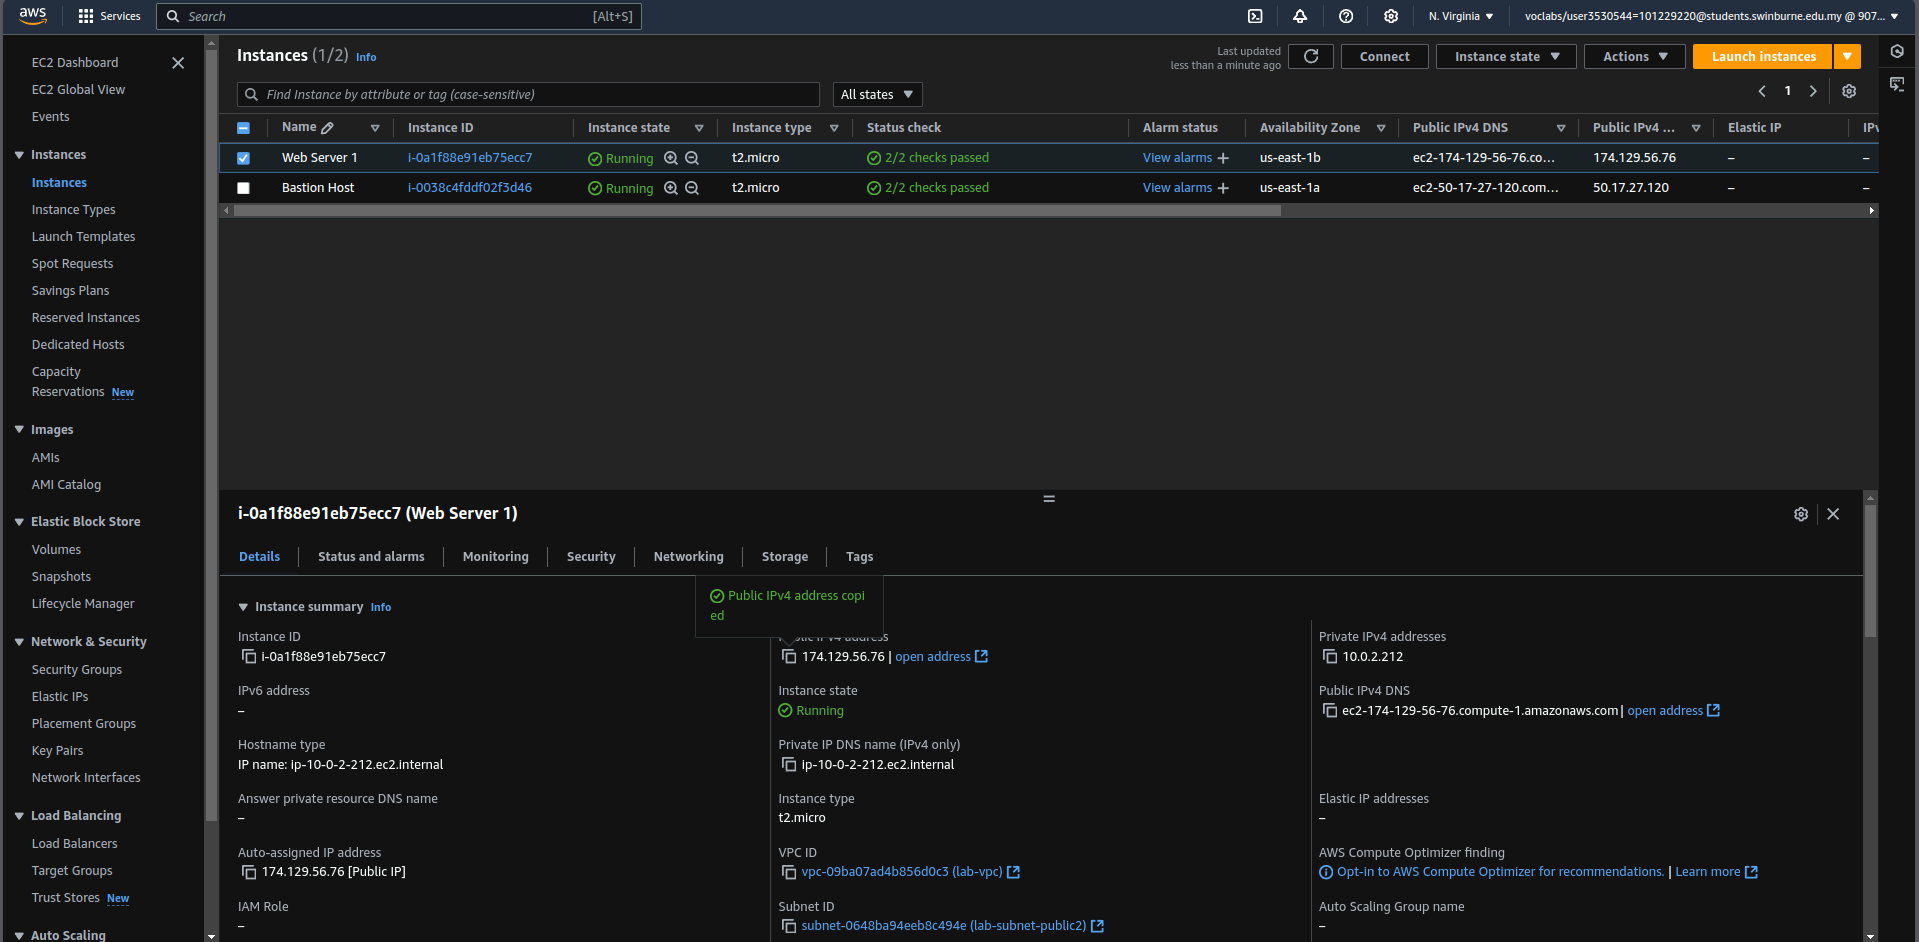
\includegraphics[width=5.8in]{pics/15a.png}
    }
    

    {\centering
    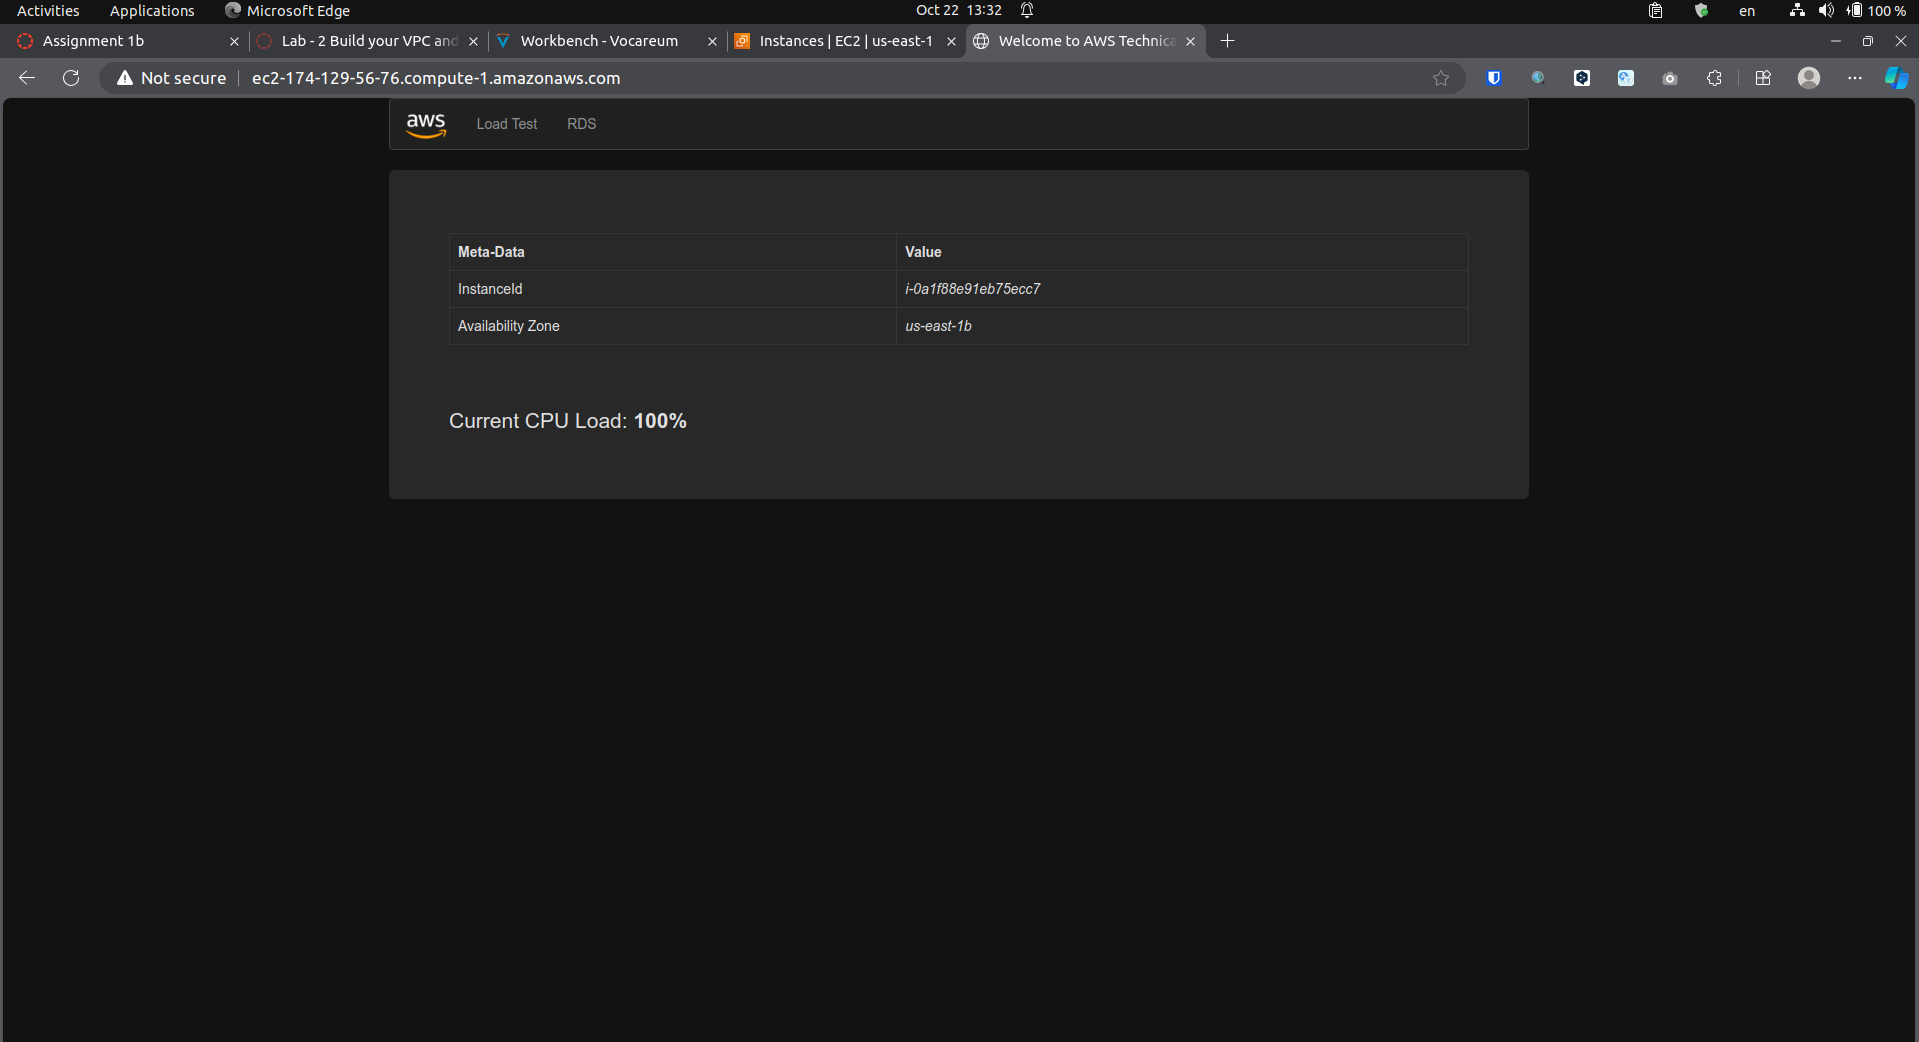
\includegraphics[width=5.8in]{pics/15b.png}
    }
    
        
\end{enumerate}

\newpage

\noindent\underline{Test Instance}

\vspace{0.5cm}

\begin{enumerate}[resume]
    \item Paste screenshot$($s$)$ of the \textbf{Instances} screen (show your running test server and the IP address)\\
    \vspace{-0.02mm}

    
    \item Paste screenshot$($s$)$ of the \textbf{terminal (e.g. Putty)} screen (show ping results)\\
    \vspace{5mm}    
    
        
\end{enumerate}


\end{document}

